%Version 3.1 December 2024
% See section 11 of the User Manual for version history
%
%%%%%%%%%%%%%%%%%%%%%%%%%%%%%%%%%%%%%%%%%%%%%%%%%%%%%%%%%%%%%%%%%%%%%%
%%                                                                 %%
%% Please do not use \input{...} to include other tex files.       %%
%% Submit your LaTeX manuscript as one .tex document.              %%
%%                                                                 %%
%% All additional figures and files should be attached             %%
%% separately and not embedded in the \TeX\ document itself.       %%
%%                                                                 %%
%%%%%%%%%%%%%%%%%%%%%%%%%%%%%%%%%%%%%%%%%%%%%%%%%%%%%%%%%%%%%%%%%%%%%

%%\documentclass[referee,sn-basic]{sn-jnl}% referee option is meant for double line spacing

%%=======================================================%%
%% to print line numbers in the margin use lineno option %%
%%=======================================================%%

%%\documentclass[lineno,pdflatex,sn-basic]{sn-jnl}% Basic Springer Nature Reference Style/Chemistry Reference Style

%%=========================================================================================%%
%% the documentclass is set to pdflatex as default. You can delete it if not appropriate.  %%
%%=========================================================================================%%

%%\documentclass[sn-basic]{sn-jnl}% Basic Springer Nature Reference Style/Chemistry Reference Style

%%Note: the following reference styles support Namedate and Numbered referencing. By default the style follows the most common style. To switch between the options you can add or remove Numbered in the optional parenthesis. 
%%The option is available for: sn-basic.bst, sn-chicago.bst%  
 
%%\documentclass[pdflatex,sn-nature]{sn-jnl}% Style for submissions to Nature Portfolio journals
%%\documentclass[pdflatex,sn-basic]{sn-jnl}% Basic Springer Nature Reference Style/Chemistry Reference Style
\documentclass[pdflatex,sn-mathphys-num]{sn-jnl}% Math and Physical Sciences Numbered Reference Style
%%\documentclass[pdflatex,sn-mathphys-ay]{sn-jnl}% Math and Physical Sciences Author Year Reference Style
%%\documentclass[pdflatex,sn-aps]{sn-jnl}% American Physical Society (APS) Reference Style
%%\documentclass[pdflatex,sn-vancouver-num]{sn-jnl}% Vancouver Numbered Reference Style
%%\documentclass[pdflatex,sn-vancouver-ay]{sn-jnl}% Vancouver Author Year Reference Style
%%\documentclass[pdflatex,sn-apa]{sn-jnl}% APA Reference Style
%%\documentclass[pdflatex,sn-chicago]{sn-jnl}% Chicago-based Humanities Reference Style

%%%% Standard Packages
%%<additional latex packages if required can be included here>

\usepackage{graphicx}%
\usepackage{multirow}%
\usepackage{amsmath,amssymb,amsfonts}%
\usepackage{amsthm}%
\usepackage{mathrsfs}%
\usepackage[title]{appendix}%
\usepackage{xcolor}%
\usepackage{textcomp}%
\usepackage{manyfoot}%
\usepackage{booktabs}%
%%===============================================================%%
%% Revision mark-up switch.                                       %%
%%   \revmarkstrue   prints every passage changed in this          %%
%%                   revision in colour and shows the note below.  %%
%%   \revmarksfalse  produces the identical text with no colour    %%
%%                   and no note: the clean copy.                  %%
%% Nothing else differs between the two versions.                  %%
%%===============================================================%%
\definecolor{revblue}{RGB}{0,70,190}%
\newif\ifrevmarks%
\revmarksfalse%     <-- change to \revmarkstrue for the marked copy
\newcommand{\revmark}[1]{\ifrevmarks\textcolor{revblue}{#1}\else#1\fi}%
\usepackage{algorithm}%
\usepackage{algorithmicx}%
\usepackage{algpseudocode}%
\usepackage{listings}%
\usepackage{placeins}%
\usepackage{multirow}
\usepackage{amsthm,amsmath}
\usepackage{lineno}
\usepackage{graphicx}
\graphicspath{ {./images/} }
\usepackage{rotating}
\usepackage{multirow}%
\usepackage{graphicx}%
\usepackage{multirow}%
\usepackage{amsmath,amssymb,amsfonts}%
\usepackage{amsthm}%
\usepackage{mathrsfs}%
\usepackage[title]{appendix}%
\usepackage{xcolor}%
\usepackage{textcomp}%
\usepackage{manyfoot}%
\usepackage{booktabs}%
\usepackage{algorithm}%
\usepackage{algorithmicx}%
\usepackage{algpseudocode}%
\usepackage{listings}%
\usepackage{natbib}%
\usepackage{array}%
\usepackage{rotating}%
\usepackage[T1]{fontenc}%
\usepackage{lmodern}%
\usepackage[utf8]{inputenc}%
\usepackage{CJKutf8}%
\usepackage{longtable}%
\usepackage{rotating}%
\usepackage{multirow}%
\usepackage{booktabs}
\usepackage{hyperref}
\usepackage{ragged2e}
\usepackage{caption}
\graphicspath{{./images/}}
%\linenumbers
%%%%

%%%%%=============================================================================%%%%
%%%%  Remarks: This template is provided to aid authors with the preparation
%%%%  of original research articles intended for submission to journals published 
%%%%  by Springer Nature. The guidance has been prepared in partnership with 
%%%%  production teams to conform to Springer Nature technical requirements. 
%%%%  Editorial and presentation requirements differ among journal portfolios and 
%%%%  research disciplines. You may find sections in this template are irrelevant 
%%%%  to your work and are empowered to omit any such section if allowed by the 
%%%%  journal you intend to submit to. The submission guidelines and policies 
%%%%  of the journal take precedence. A detailed User Manual is available in the 
%%%%  template package for technical guidance.
%%%%%=============================================================================%%%%

%% as per the requirement new theorem styles can be included as shown below
\theoremstyle{thmstyleone}%
\newtheorem{theorem}{Theorem}%  meant for continuous numbers
%%\newtheorem{theorem}{Theorem}[section]% meant for sectionwise numbers
%% optional argument [theorem] produces theorem numbering sequence instead of independent numbers for Proposition
\newtheorem{proposition}[theorem]{Proposition}% 
%%\newtheorem{proposition}{Proposition}% to get separate numbers for theorem and proposition etc.

\theoremstyle{thmstyletwo}%
\newtheorem{example}{Example}%
\newtheorem{remark}{Remark}%

\theoremstyle{thmstylethree}%
\newtheorem{definition}{Definition}%

\raggedbottom
%%\unnumbered% uncomment this for unnumbered level heads

\begin{document}

\title[Interpretable Hardness Prediction in Graphene-Added Si$_3$N$_4$ Ceramics]{Interpretable Small-Data Hardness Prediction in Graphene-Added Si$_3$N$_4$ Ceramics via Rule-Based Ceramic Informatics}

%%=============================================================%%
%% GivenName	-> \fnm{Joergen W.}
%% Particle	-> \spfx{van der} -> surname prefix
%% FamilyName	-> \sur{Ploeg}
%% Suffix	-> \sfx{IV}
%% \author*[1,2]{\fnm{Joergen W.} \spfx{van der} \sur{Ploeg} 
%%  \sfx{IV}}\email{iauthor@gmail.com}
%%=============================================================%%

\author[1]{\fnm{Yunus E.} \sur{Salcan}}\email{yunusemresalcan@gmail.com,https://orcid.org/0009-0000-1935-6902}

\author[2]{\fnm{Emre} \sur{Bal*}}\email{emrebal@akdeniz.edu.tr, https://orcid.org/0000-0003-1052-7749}

\author[2,3]{\fnm{Sadettin Y.} \sur{Ugurlu}}\email{s.yavuz.ugurlu@gmail.com, https://orcid.org/0000-0001-9589-0269}

\affil[1]{\orgdiv{Department of Science}, \orgname{Akdeniz University}, \orgaddress{\street{Dumlupinar Bulvari}, \city{Antalya}, \postcode{07058}, \country{Turkey}}}
\affil[2]{\orgdiv{Department of Materials Science and Engineering, Faculty of Engineering}, \orgname{Akdeniz University}, \orgaddress{\street{Dumlupinar Bulvari}, \city{Antalya}, \postcode{07058}, \country{Turkey}}}
\affil[3]{\orgname{Novexus Ltd}, \orgaddress{\country{Turkey}}}


%%==================================%%
%% Sample for unstructured abstract %%
%%==================================%%

\abstract{
Accurate prediction of Vickers hardness in graphene-added Si$_3$N$_4$ ceramics remains challenging because hardness depends on coupled composition--processing--structure relationships, while available experimental datasets are small and expensive to expand. This study develops an interpretable machine-learning framework centred on a tuned RuleFit model using an 82-sample literature-derived dataset of graphene-added Si$_3$N$_4$ ceramics. The workflow benchmarks RuleFit against XGBoost models trained with original and physically engineered features, regularised linear baselines, Few-Shot KNN, and a compact neural network. Performance was evaluated using fixed 80/20 and 70/30 train--test splits, followed by a 30-replicate random-split stability analysis.

\revmark{On the fixed 70/30 split, RuleFit (Tuned) achieved the best split-specific performance, with $R^2 = 0.854$, RMSE $= 1.955$ GPa, and MAE $= 1.477$ GPa. Across 30 random splits, for which the configuration was fixed in advance, RuleFit remained statistically comparable to the strongest XGBoost baselines and significantly outperformed Few-Shot KNN (Cohen's $d_z > 1.1$; Bonferroni-corrected $p < 0.001$), demonstrating that interpretable rule-based modelling can approach black-box accuracy under small-data conditions. Repeating the whole protocol with a strictly leakage-free hyperparameter search inside each training partition gave statistically indistinguishable results (paired $\Delta R^2 = -0.009$, 95\% CI $[-0.048, +0.029]$), confirming that the reported performance does not depend on the configuration choice. A leave-one-reference-out analysis across sixteen literature sources showed that cross-source generalisation is substantially more challenging than random-split evaluation (pooled $R^2 = 0.39$--$0.49$), highlighting the impact of literature-source heterogeneity.}

RuleFit and SHAP analyses consistently identified graphene content/type, sintering pressure, Si$_3$N$_4$ content, and relative density as the most influential predictors, consistent with established ceramic processing--property relationships. Sample-level case studies further demonstrated that activated RuleFit rules provide transparent local explanations broadly consistent with SHAP and LIME. Overall, the proposed framework delivers competitive small-data hardness prediction while translating complex model behaviour into explicit processing--property rules. Although particularly valuable for graphene-added Si$_3$N$_4$ ceramics, the limited dataset size and reliance on post-sintering descriptors require cautious interpretation until validated with independent experimental data. The cleaned dataset, feature-generation pipeline, model-training scripts, and random seeds are publicly available at \url{https://github.com/Yemresalcan/si3n4_graphene_rulefit}.
}


\keywords{Vickers hardness, Si$_3$N$_4$ ceramics, graphene, RuleFit, interpretable machine learning, ceramic informatics, small-data modelling, SHAP, LIME, feature engineering}


\maketitle

\ifrevmarks
\noindent\textcolor{revblue}{\textbf{Note to the reviewer and editor:} all passages modified in this revision are printed in this colour. Text in black is unchanged with respect to the previous version. Rebuilt tables and redrawn figures are indicated by a coloured caption. The accepted, typeset version of the article is produced from the identical source with the mark-up switch turned off, so no colour reaches the published text.}\bigskip
\fi



\section{Introduction}
\revmark{Silicon nitride (Si$_3$N$_4$) ceramics are among the most important advanced structural ceramics because they combine high hardness, high fracture toughness, low density, good thermal-shock resistance, oxidation resistance, and chemical stability under demanding service conditions \cite{petzow2002silicon, klemm2010silicon, riley2000silicon, qadir2018effect, govindasamy2024role}. These properties make Si$_3$N$_4$ attractive for cutting tools, bearings, automotive engine components, wear-resistant parts, and high-temperature structural applications \cite{petzow2002silicon, klemm2010silicon, riley2000silicon, qadir2018effect, govindasamy2024role}. In recent years, graphene and graphene-derived nanomaterials have been incorporated into ceramic matrices to further modify mechanical, tribological, electrical, and thermal performance \cite{zhu2010graphene, soldano2010production, miranzo2017bulk}. In graphene-added Si$_3$N$_4$ ceramics, however, the final hardness is not governed by a single compositional variable; instead, it emerges from the combined effects of graphene type and content, sintering temperature, sintering pressure, holding time, additives, density, and phase composition \cite{qadir2024predicting, balazsi2003preparation, wang2016synthesis, ramirez2014extraordinary, yang2002microstructure, german2009liquid}. This multi-factor dependence makes experimental optimisation difficult because a change that improves one property may reduce densification or hardness. Therefore, reliable hardness prediction is necessary.}

\revmark{Reliable hardness prediction is vital because Vickers hardness is directly related to wear resistance, contact-damage tolerance, indentation response, and the suitability of a ceramic component for load-bearing or tribological applications \cite{petzow2002silicon, qadir2018effect, ullner2001hardness}. If hardness can be estimated before or immediately after processing from available composition, processing, and microstructural descriptors, researchers can reduce the number of trial-and-error sintering experiments, prioritise promising graphene contents, identify suitable pressure--temperature windows, and avoid processing routes that are likely to produce porous or mechanically weak samples \cite{qadir2024predicting, balazsi2003preparation,chen2016xgboost}. This is particularly important for graphene-reinforced Si$_3$N$_4$, where low graphene additions may improve or preserve performance, whereas excessive graphene can promote agglomeration, reduce density, and decrease hardness~ \cite{qadir2024predicting, ramirez2014extraordinary}. Therefore, hardness prediction can support both materials screening and process--structure--property understanding. Thus, hardness prediction has become a practical materials-design problem rather than only a post-test measurement.}

As a practical materials-design problem, hardness prediction has increasingly been addressed using data-driven and machine-learning methods. In ceramic and materials-science applications, artificial neural networks, Gaussian-process-based approaches, random forests, gradient boosting, support vector regression, and XGBoost have been used to model nonlinear relationships between processing variables and target properties~ \cite{qu2019ultra, deng2018optimization, liu2020machine, butler2018machine, schmidt2019recent, ward2016general, ramprasad2017machine}. For graphene-added Si$_3$N$_4$ ceramics specifically, Qadir et al.~ \cite{qadir2024predicting} compiled a literature-derived dataset and demonstrated that XGBoost could predict Vickers hardness with strong accuracy while identifying sintering pressure, sintering time, density, graphene content, and graphene type as influential factors. Their study established an important machine-learning baseline for this small but experimentally valuable materials system. Beyond predictive modelling, explainable artificial intelligence methods such as SHAP and LIME have also become widely used to interpret complex models and assign feature-level contributions to individual predictions \cite{lundberg2017unified, ribeiro2016should}. However, this progress has also exposed important limitations in current hardness-prediction studies.

Current hardness-prediction studies still have important limitations. First, strong black-box models such as XGBoost can provide accurate predictions. Still, they do not naturally express the learned processing--property relationships as simple rules that materials researchers can inspect and reuse \cite{qadir2024predicting, butler2018machine, lundberg2017unified}. Second, graphene-added Si$_3$N$_4$ datasets remain small, meaning that single train--test splits can overstate model performance and may not adequately reflect split-to-split stability. Third, some descriptors, such as density and $\alpha$/$\beta$ phase content, are post-sintering variables; therefore, models using the full feature set should be interpreted carefully as post-synthesis or process--structure--property models rather than purely pre-synthesis design tools \cite{qadir2024predicting}. Fourth, feature engineering is often limited, even though physically meaningful interaction terms such as sintering intensity, sintering dose, graphene aspect ratio, or additive ratios may better represent the coupled effects of processing and composition. Finally, many studies report global feature importance but provide limited sample-level explanations, making it difficult to understand why a specific high- or low-hardness ceramic is predicted in a particular way. Addressing these limitations requires a model that is not only accurate but also interpretable, stable under small-data conditions, and reproducible.

\revmark{To address these limitations, this study develops an interpretable and robust hardness-prediction framework for graphene-added Si$_3$N$_4$ ceramics using a tuned RuleFit model and a literature-derived dataset of 82 experimentally characterised samples. The central aim is not only to predict Vickers hardness, but also to determine whether competitive predictive performance can be achieved with a model whose decisions can be inspected through physically meaningful rules. For this purpose, RuleFit is benchmarked against XGBoost models trained with original and engineered features, regularised linear baselines, few-shot KNN, and a compact neural network under fixed 80/20 and 70/30 train--test splits, followed by a 30-replicate random-split stability analysis. Unlike purely black-box models, RuleFit combines tree-derived nonlinear rules with a sparse linear model, allowing individual predictions to be traced through human-readable rule activations \cite{friedman2008predictive}. In parallel, SHAP and LIME are used to examine whether the same predictions are explained consistently from global and local interpretability perspectives \cite{lundberg2017unified, ribeiro2016should}. The methodological contribution is therefore fourfold: first, to evaluate whether an interpretable RuleFit model can remain competitive with XGBoost-based black-box baselines in a small ceramic dataset; second, to introduce physically motivated engineered descriptors that represent coupled composition--processing effects such as sintering intensity, sintering dose, graphene aspect ratio, and additive balance; third, to assess split-level robustness and reduce the risk of over-interpreting a single favorable partition; and fourth, to connect predictive performance with ceramic processing--property interpretation through RuleFit rules, SHAP, LIME, and sample-level case studies. By linking graphene content and type, sintering pressure, Si$_3$N$_4$ content, relative density, and engineered processing descriptors to transparent rules, this work provides a cautious but practically useful step toward interpretable machine learning for ceramic hardness prediction. From a materials-science perspective, the main value of the proposed framework is not limited to numerical prediction. By translating the influence of graphene content, sintering pressure, relative density, phase-related descriptors, and engineered processing terms into explicit rules and feature attributions, the study provides a structure--processing--property interpretation layer for a ceramic system in which further experimental expansion is expensive. Therefore, the work is positioned as a ceramic-informatics contribution that complements conventional experimental optimisation rather than replacing it.}

\section{Materials and Methods}
The proposed methodology integrates dataset construction, leakage-aware preprocessing, physically motivated feature engineering, model benchmarking, repeated-split stability analysis, and interpretable rule extraction into a single reproducible workflow for Vickers hardness prediction in graphene-added Si$_3$N$_4$ ceramics. The framework was designed to address three connected objectives: (i) to construct a transparent feature space from literature-reported experimental observations, (ii) to compare an interpretable RuleFit model with strong machine-learning baselines, and (iii) to evaluate whether the resulting predictions can be explained through physically meaningful global and local interpretation methods. For this purpose, RuleFit rule activations, SHAP, and LIME were used alongside conventional regression metrics so that model performance could be assessed not only by predictive accuracy, but also by robustness, transparency, and consistency with established ceramic processing--property relationships. The resulting workflow links model benchmarking (Tables~\ref{tab:80_20}--\ref{tab:ttest}), global feature analysis (Figs.~\ref{fig:corr_heatmap}--\ref{fig:rulefit_rules}), data-structure visualisation (Fig.~\ref{fig:pca_tsne}), and sample-level interpretability (Table~\ref{tab:case_overview} and Fig.~\ref{fig:shap_waterfall}) into a single evaluation strategy.



\subsection{Development of the Interpretable Hardness Prediction Framework}

The dataset used in this study consists of 82 experimental observations of graphene-added Si$_3$N$_4$ ceramics compiled from the literature \cite{qadir2024predicting}. The target variable is Vickers hardness measured in GPa, ranging from 0.46 to 27.00~GPa with a mean of 14.71~GPa. Each sample is described by 21 input features covering graphene properties (type, weight fraction, thickness, surface area), sintering additive characteristics (type and content of two additives), milling conditions (type and duration), sintering parameters (technique, temperature, time, pressure), and post-sintering properties (density, $\alpha$- and $\beta$-Si$_3$N$_4$ phase content, and indentation load).

Categorical features (type of graphene, type of sintering additive 1 and 2, milling type, and sintering technique) were converted into numeric representations using target encoding. Because target encoding can leak response information if it is fitted globally, it was treated as a split-dependent preprocessing step: encoders were fitted only on the training subset and then applied unchanged to the corresponding validation or test subset. During cross-validation-based optimisation, categorical encoders were re-fitted inside each training fold and never on the held-out fold. This design prevents the test-set hardness distribution from influencing encoded categorical values. A reference/source label was retained only for traceability and was excluded from the predictive feature set because it may encode literature-source-specific bias rather than transferable material behavior. After encoding and source-label exclusion, the original feature set contained 22 numeric variables.

To capture physically meaningful interactions, eight additional engineered features were derived from the existing variables: (i) graphene aspect ratio (surface area / thickness), (ii) graphene volume proxy (wt.\% $\times$ thickness $\times$ surface area), (iii) sintering energy (temperature $\times$ time), (iv) sintering intensity (temperature $\times$ pressure), (v) sintering dose (temperature $\times$ time $\times$ pressure), (vi) total additive content (additive 1 + additive 2), (vii) additive ratio (additive 1 / additive 2), and (viii) Si$_3$N$_4$-to-additive ratio (Si$_3$N$_4$ wt.\% / total additive). These variables are used as empirical morphology and process proxies rather than direct physical quantities with strict dimensional interpretation. In particular, sintering kinetics are governed by strongly nonlinear mechanisms, including Arrhenius-type temperature dependence and creep- or diffusion-controlled densification laws, so simple multiplicative terms such as sintering intensity or sintering dose should not be read as literal measures of the thermodynamic driving force for densification. They are empirical interaction proxies whose only claim is that they expose coupled temperature--time--pressure effects in a form that a sparse model can select; accordingly, the coefficient signs attached to these composite terms in the fitted models are interpreted as data-driven associations rather than as statements about the underlying physical mechanisms. Their purpose is to expose coupled effects that may be difficult for a small-data model to learn from the original variables alone. For example, sintering intensity and sintering dose approximate the combined thermal--mechanical driving force for densification, whereas the Si$_3$N$_4$-to-additive ratio and total additive content represent matrix--additive balance. Similarly, the graphene aspect ratio and the graphene volume proxy describe morphology-related effects that may influence dispersion, interfacial contact, agglomeration tendency, and load transfer. For ratio-based descriptors, a small denominator offset (0.01) was used to avoid undefined values when additive content or graphene thickness was zero. The complete feature set after engineering consists of 30 numeric features.

The dataset was split into training and test sets using two configurations: 80/20 (66 training, 16 test) and 70/30 (57 training, 25 test). In both cases, a fixed random seed (random\_state = 42) was used to ensure reproducibility. For every split, preprocessing steps that learn parameters from the data, including target encoding and standardisation where applicable, were fitted on the training subset only and transferred unchanged to the held-out test subset. Engineered features were computed from the available input variables without using the hardness target. This workflow was used to keep the held-out test data independent from model fitting and model selection.

\revmark{The proposed interpretable framework is built upon the RuleFit algorithm \cite{friedman2008predictive}, which combines an ensemble of decision trees with a sparse linear model to produce human-readable prediction rules. In RuleFit, the trees generate candidate rules (conjunctions of feature thresholds), which are then used as binary features in a regularised linear model (Lasso). The final model is a sum of linear terms and weighted rule activations, making every prediction fully traceable.}

\revmark{Hyperparameter tuning of RuleFit was performed by a grid search over \texttt{tree\_size} $\in \{2, 3, 4, 6, 8\}$ and \texttt{max\_rules} $\in \{50, 100, 200, 500\}$. The selected configuration was \texttt{tree\_size} = 6 and \texttt{max\_rules} = 500, referred to as \textit{RuleFit (Tuned)} throughout the paper, and the untuned configuration (\texttt{tree\_size} = 4, \texttt{max\_rules} = 100) is referred to as \textit{RuleFit (Default)}. This single configuration was then held fixed for every subsequent experiment, including all 30 repeated partitions, the leave-one-reference-out analysis and the pre-synthesis ablation; it was never re-selected per partition, so each of those partitions supplies an independent held-out set for a configuration chosen in advance. Because a single fixed configuration nevertheless conditions the reported performance to some degree, Section~\ref{sec:selection} measures that dependence directly rather than assuming it, by repeating the entire protocol with the grid search confined to the training data of every individual partition.}

\revmark{The reason for retaining this protocol rather than replacing it deserves a direct statement. The purpose of the study is a head-to-head comparison against the published XGBoost workflow of Qadir et al.~\cite{qadir2024predicting} on the same dataset, and that comparison is only meaningful if both sides are evaluated under the same conditions. Altering the evaluation protocol --- even in a direction that would be methodologically preferable in isolation --- would change the conditions on one side only and would introduce a bias against the reference method. For the same reason no additional samples were introduced: enlarging the dataset would break comparability with the baseline study and would confound any observed difference with a change in data. The dataset limitation is instead addressed statistically, by repeating the evaluation over 30 random partitions of the same data and reporting effect sizes, confidence intervals and corrected $p$ values (Tables~\ref{tab:stability} and~\ref{tab:ttest}), so that the comparison is made as informative as the available evidence allows while the protocol itself remains unchanged. Every element of the workflow, including the selection step described above, is available in the public repository so that any reader can re-execute it and verify these statements.}


\subsection{Performance Evaluation and Robustness Assessment}

To assess the performance of the trained machine learning models, multiple evaluation metrics were used to quantify predictive accuracy and error. The evaluation framework was designed to assess the reliability of the models in predicting Vickers hardness. The following statistical metrics were used for performance evaluation:  

\paragraph{Coefficient of Determination ($R^2$)}  
The $R^2$ score measures the proportion of variance in the observed data that is explained by the model’s predictions. A value closer to 1 indicates that the model explains a larger proportion of the variance in the observed outcomes, whereas lower values indicate weaker predictive performance. The $R^2$ metric is particularly useful for understanding the overall explanatory power of the model.  

\paragraph{Mean Absolute Error (MAE)}
MAE measures the average absolute difference between the experimentally measured hardness values and the corresponding model predictions. Unlike RMSE, MAE does not square the residuals and is therefore less dominated by a small number of large errors. It is reported in GPa and provides a direct estimate of the typical prediction deviation:

\begin{equation}
MAE = \frac{1}{n} \sum_{i=1}^{n} |y_i - \hat{y}_i|
\end{equation}

where $y_i$ is the measured Vickers hardness, $\hat{y}_i$ is the predicted hardness, and $n$ is the number of samples.

\paragraph{Root Mean Squared Error (RMSE)}  
\revmark{RMSE quantifies the model’s predictive accuracy by calculating the square root of the mean squared differences between predicted and actual values. It penalises larger errors more than smaller ones, making it a suitable metric for evaluating models where significant deviations in predictions are undesirable. RMSE is computed as:}

\begin{equation}
\label{eq:rmse}
RMSE = \sqrt{\frac{1}{n} \sum_{i=1}^{n} (y_i - \hat{y}_i)^2}
\end{equation}

where $y_i$ represents the actual values, $\hat{y}_i$ represents the predicted values, and $n$ is the total number of data points.  

In addition to testing set performance, the RMSE has been computed for the training set to evaluate how well the model fits the training data and to identify potential overfitting. The RMSE for the training set reflects the average prediction error during model fitting and provides a baseline for comparison against validation and test performance. A significantly lower RMSE on the training set relative to the test set may indicate overfitting, whereas comparable values suggest generalizability. RMSE is calculated using Eq.~\eqref{eq:rmse}, where predictions $\hat{y}_i$ are generated for the training set samples.


\paragraph{Adjusted Coefficient of Determination ($R^2_{\text{adj}}$)}  
\revmark{While the standard $R^2$ score quantifies how well the model captures variance in the data, it does not account for the number of predictors used in the model. Given that the proposed framework incorporates 30 input features (22 original + 8 engineered), the adjusted $R^2$ ($R^2_{\text{adj}}$) is also reported to correct for potential overfitting. Adjusted $R^2$ provides a more accurate assessment of the model’s explanatory power on the training set by penalising excessive use of features that do not significantly contribute to prediction. It is computed as:}

\begin{equation}
\label{eq:adjusted_r2}
R^2_{\text{adj}} = 1 - \left( \frac{(1 - R^2)(n - 1)}{n - p - 1} \right)
\end{equation}

where $n$ is the number of observations, $p$ is the number of predictors (features), and $R^2$ is the unadjusted coefficient of determination. This metric was calculated for the training set to ensure that model complexity is justified by meaningful predictive power.


\subsection{Framework Interpretability, Feature Attribution, and Statistical Analysis}

\paragraph{Correlation-Based Feature Clustering}
Hierarchical clustering of all 30 engineered features together with the target variable (Vickers hardness) was performed using Pearson correlation as the similarity measure. The distance between two variables was defined as $d = 1 - |\rho|$, where $\rho$ is the Pearson correlation coefficient. Average linkage was applied to the resulting correlation-based distance matrix to produce the dendrogram. Including the target in the clustering allows visual identification of which feature families are most correlated with hardness.

\paragraph{Global Feature Importance and Attribution Analysis}
\revmark{Feature importance was assessed from two complementary perspectives. First, the retained linear terms and extracted Boolean rules from RuleFit were inspected to identify variables that enter the sparse interpretable model. Second, SHAP (SHapley Additive exPlanations) values were computed via TreeExplainer to provide attribution across all 25 test-set samples of the fixed 70/30 split \cite{lundberg2017unified}. To keep the interpretability analysis independent of the randomised hyperparameter search used in the benchmark, the SHAP, LIME and case-study results were produced with a single fixed XGBoost configuration (\texttt{n\_estimators} = 300, \texttt{max\_depth} = 5, \texttt{learning\_rate} = 0.05, \texttt{subsample} = \texttt{colsample\_bytree} = 0.8), referred to hereafter as the \textit{interpretability XGBoost model}. This is not the same fit as the \textit{XGBoost (Extra Features, Tuned)} row of the benchmark tables: on the same 70/30 partition the interpretability model reaches $R^2 = 0.809$ and MAE~=~1.746~GPa, against $R^2 = 0.835$ and MAE~=~1.599~GPa for the tuned benchmark model. All XGBoost-based attributions, including every value quoted for samples P1--P5, refer to the interpretability model, and the benchmark tables refer to the tuned model; the two are reported separately and are not interchanged.}

\paragraph{Sample-Level Local Interpretability}
Local explanations for five selected test samples were generated using three methods: (i) RuleFit rule activation (which rules fire for a given sample and how they contribute to the prediction), (ii) SHAP values (XGBoost), and (iii) LIME (Local Interpretable Model-agnostic Explanations), which fits a locally weighted linear model around each prediction \cite{ribeiro2016should}. The five samples were selected from the 25-sample test set to represent a range of prediction accuracy: two high-accuracy predictions ($|$error$|$ $<$ 0.15 GPa), two moderate-accuracy predictions ($|$error$|$ $\approx$ 0.85 GPa), and one challenging case ($|$error$|$ = 4.46 GPa).

\paragraph{Repeated-Split Statistical Significance Analysis}
The stability of each model across 30 random splits was evaluated using one-tailed paired Student's $t$-tests (significance level $\alpha = 0.05$). The one-tailed formulation was used to address a directional question: whether the interpretable RuleFit model achieved a higher R$^2$ or lower error than each comparator. For R$^2$, the null hypothesis is that RuleFit (Tuned) performs no better than the comparison model; for MAE and RMSE, the null hypothesis is that RuleFit (Tuned) is no lower than the comparison model. Because repeated random splits share observations and are not fully independent, these tests are interpreted as exploratory rather than definitive hypothesis tests. The critical value for 29 degrees of freedom at $\alpha = 0.05$ (one-tailed) is $t_\text{critical} = 1.699$. To account for the multiplicity of the 18 pairwise comparisons (six comparators $\times$ three metrics), Bonferroni- and Holm-corrected $p$-values were additionally computed, and paired effect sizes (Cohen's $d_z$) together with 95\% confidence intervals of the paired metric differences are reported alongside the uncorrected $p$-values. The corrected values are provided in the public repository, and the interpretation in the main text emphasises effect sizes and confidence intervals rather than single uncorrected $p$-values.

\paragraph{Source-Level and Pre-Synthesis Sensitivity Analyses}
Because the dataset aggregates measurements from sixteen literature sources, two additional sensitivity analyses were performed. First, a leave-one-reference-out (LORO) validation was conducted: in each of the sixteen folds, all samples originating from one literature source were held out as the test set, target encoders were re-fitted on the remaining training samples only, and pooled out-of-fold predictions were used to compute global R$^2$, MAE, and RMSE. This protocol tests whether the models generalise to entirely unseen experimental sources rather than to unseen samples from partially seen sources. Second, a pre-synthesis ablation was performed in which the post-sintering descriptors (relative density and $\alpha$-/$\beta$-Si$_3$N$_4$ phase content) were removed from the feature set, and the 30-replicate random-split protocol was repeated with the remaining 27 features. This ablation quantifies how much predictive performance depends on descriptors that are only available after sintering.

 






\subsection{Comparison with the Published XGBoost Baseline}
\label{sec:method_comparison}

The comparative design was anchored to the XGBoost modelling strategy reported by Qadir et al.~\cite{qadir2024predicting}. Their study used the same 82-sample graphene-added Si$_3$N$_4$ dataset and reported high predictive accuracy for Vickers hardness, making it the most relevant published state-of-the-art reference for this dataset. In the present manuscript, \textit{XGBoost (Default Features, Tuned)} is a reimplemented baseline following that modelling strategy, rather than a direct reproduction of the numerical results reported by Qadir et al. It uses the original encoded feature set and RandomizedSearchCV hyperparameter optimisation (50 iterations with 5-fold cross-validation), and is marked with an asterisk in the Results section.

A second XGBoost configuration, \textit{XGBoost (Extra Features, Tuned)}, was included to test whether the eight physically motivated engineered features improve the black-box baseline. This model should be interpreted as an extended in-house benchmark rather than the original published baseline. The purpose of including both XGBoost variants is to separate two questions: (i) whether RuleFit remains competitive against the published high-performing XGBoost reference, and (ii) whether the engineered 30-feature representation changes the ranking of the strongest models.

The following model configurations are included in the comparison:

\begin{enumerate}
    \item \textbf{XGBoost (Default Features, Tuned)$^{*}$}: XGBoost with the original 22 numeric features and RandomizedSearchCV optimisation (50 iterations, 5-fold CV), reimplemented following the published state-of-the-art strategy of Qadir et al.~\cite{qadir2024predicting}.
    \item \textbf{XGBoost (Extra Features, Tuned)}: XGBoost with all 30 features (22 original + 8 engineered) and the same RandomizedSearchCV optimisation, used to evaluate the effect of feature engineering.
    \item \textbf{ElasticNet}: Elastic net regularised linear regression (L1 + L2, $\alpha$ = 1.0, $l_1$-ratio = 0.5) applied to standardised 30-feature data.
    \item \textbf{RuleFit (Tuned)}: RuleFit with optimised hyperparameters (\texttt{tree\_size} = 6, \texttt{max\_rules} = 500) trained on the 30-feature data.
    \item \textbf{RuleFit (Default)}: RuleFit with default hyperparameters (\texttt{tree\_size} = 4, \texttt{max\_rules} = 100) trained on the 30-feature data.
    \item \textbf{DNN Small (32--16)}: A two-hidden-layer multilayer perceptron with 32 and 16 neurons, trained for up to 2000 epochs with early stopping and applied to standardised 30-feature data.
\end{enumerate}

Few-Shot KNN was included as a small-data reference in the repeated-split analysis and learning-curve experiments. It used three distance-weighted nearest neighbours with Euclidean distance on standardised 30-feature data. It is reported in the stability analysis rather than in the fixed-split tables to keep the primary comparison focused on RuleFit and the XGBoost baselines.

Each model was evaluated on two fixed train--test splits (80/20 and 70/30, both with random\_state = 42) and on 30 random 70/30 splits (random\_state = 0, 1, \ldots, 29) to assess stability. Performance is reported as R$^2$, mean absolute error (MAE, in GPa), and root mean squared error (RMSE, in GPa).






\section{Results and Discussion}
\revmark{The results are presented as a combined assessment of accuracy, robustness, interpretability, and physical consistency. The first objective is to determine whether the proposed RuleFit-based framework can achieve predictive performance comparable to high-performing black-box baselines, particularly XGBoost, while preserving transparent rule-level explanations. The second objective is to examine whether the dominant predictors identified by the models correspond to established ceramic processing--structure--property relationships, including the effects of graphene addition, sintering pressure, relative density, and Si$_3$N$_4$ content on Vickers hardness. The third objective is to evaluate the stability of the modeling conclusions under small-data conditions, where single train--test partitions can produce overly optimistic or split-specific results. For this reason, fixed 80/20 and 70/30 splits are interpreted together with a 30-replicate random-split analysis. Finally, global feature attribution, data-structure visualisation, and sample-level case studies are used to determine whether the predictions can be explained consistently across RuleFit rules, SHAP, and LIME. This organisation allows the discussion to move from model-level benchmarking to physically interpretable prediction behaviour, thereby positioning the framework as both a predictive and explanatory tool for graphene-added Si$_3$N$_4$ hardness modelling.}


\subsection{Comparative Analysis}
\label{sec:comparative}

The predictive performance of the evaluated model configurations was first examined using a fixed 80/20 train--test split. Table~\ref{tab:80_20} reports the corresponding R$^2$, MAE, and RMSE values for all models. The asterisked XGBoost row denotes the reimplemented baseline following the published state-of-the-art strategy of Qadir et al.~\cite{qadir2024predicting}; the remaining rows are evaluated within the present workflow.

%%% TABLE 1: 80/20 SPLIT %%%

\begin{table}[h]
\footnotesize
\centering
\renewcommand{\arraystretch}{1.4}
\caption{Predictive performance of the evaluated models on the fixed 80/20 train--test split (66 training samples and 16 test samples; random\_state~$= 42$). The table reports R$^2$, mean absolute error (MAE), and root mean squared error (RMSE) for Vickers hardness prediction; MAE and RMSE are given in GPa. The best values in this split are obtained by XGBoost with engineered features ($R^2=0.822$, MAE~=~1.254~GPa, RMSE~=~1.932~GPa).}
\label{tab:80_20}
\begin{tabular}{lccc}
\hline
\textbf{Model} & \textbf{R$^2$} & \textbf{MAE (GPa)} & \textbf{RMSE (GPa)} \\ \hline
XGBoost (Default Features, Tuned)$^{*}$ & 0.819 & 1.380 & 1.948 \\
XGBoost (Extra Features, Tuned)   & 0.822 & 1.254 & 1.932 \\
ElasticNet                        & 0.677 & 1.925 & 2.604 \\
RuleFit (Tuned)                   & 0.754 & 1.642 & 2.269 \\
RuleFit (Default)                 & 0.785 & 1.484 & 2.125 \\
DNN Small (32-16)                 & 0.758 & 1.545 & 2.251 \\
\hline
\end{tabular}
\vspace{1mm}
\scriptsize{$^{*}$Reimplemented XGBoost baseline following the published state-of-the-art strategy of Qadir et al.~\cite{qadir2024predicting}.}
\end{table}
\FloatBarrier

\revmark{On the 80/20 split, the strongest result is obtained by XGBoost with engineered features, which reaches $R^2=0.822$, MAE~=~1.254~GPa, and RMSE~=~1.932~GPa (Table~\ref{tab:80_20}). The reimplemented XGBoost baseline is very close, with $R^2=0.819$, MAE~=~1.380~GPa, and RMSE~=~1.948~GPa. RuleFit does not lead this split, but the default RuleFit model remains competitive with $R^2=0.785$ and RMSE~=~2.125~GPa. Notably, the default configuration outperforms the tuned one on this partition ($R^2=0.754$, MAE~=~1.642~GPa, RMSE~=~2.269~GPa), which is the first indication that the configuration selected on the 70/30 partition does not transfer automatically to a different partition of the same data. DNN Small sits between the two RuleFit variants at $R^2=0.758$ with MAE~=~1.545~GPa, so on this split it is neither the best nor an outlier; its instability becomes visible only under repeated resampling (Table~\ref{tab:stability}). In contrast, ElasticNet gives the lowest $R^2$ value ($R^2=0.677$) together with the highest MAE (1.925~GPa) and RMSE (2.604~GPa) of the six models, indicating that a mainly linear formulation is less suitable for this correlated feature space. The spread between the best and worst $R^2$ on this partition is 0.145, which is narrow enough that the ranking should not be read as a decisive separation of model families.}

The weaker performance of the linear baseline is consistent with nonlinear and interaction-dependent relationships in the dataset. For example, the association between graphene content and hardness may depend on sintering pressure, relative density, dispersion quality, and processing route rather than following a single global linear trend. Tree-based methods and RuleFit can represent such threshold-like interactions more flexibly than an unregularised linear model. The instability of DNN Small, however, is more appropriately attributed to its high parameter-to-sample ratio and sensitivity to the small early-stopping validation subset than to an inherent limitation of neural networks for ceramic-property modelling.

The 80/20 split also shows that feature engineering slightly improves the XGBoost baseline, reducing MAE from 1.380 to 1.254~GPa and RMSE from 1.948 to 1.932~GPa. This modest improvement suggests that the engineered descriptors provide useful but not dominant additional information; most of the predictive signal is already present in the original composition, processing, and post-sintering variables.

To examine whether the model ranking changes with a larger held-out test partition, the same model configurations were then evaluated using a fixed 70/30 train--test split. The results are presented in Table~\ref{tab:70_30}.

%%% TABLE 2: 70/30 SPLIT %%%

\begin{table}[h]
\footnotesize
\centering
\renewcommand{\arraystretch}{1.4}
\caption{Predictive performance of the evaluated models on the fixed 70/30 train--test split (57 training samples and 25 test samples; random\_state~$= 42$). The table reports R$^2$, MAE, and RMSE for Vickers hardness prediction; MAE and RMSE are given in GPa. RuleFit (Tuned) gives the best split-specific performance with $R^2=0.854$, MAE~=~1.477~GPa, and RMSE~=~1.955~GPa.}
\label{tab:70_30}
\begin{tabular}{lccc}
\hline
\textbf{Model} & \textbf{R$^2$} & \textbf{MAE (GPa)} & \textbf{RMSE (GPa)} \\ \hline
XGBoost (Default Features, Tuned)$^{*}$  & 0.817 & 1.757 & 2.187 \\
XGBoost (Extra Features, Tuned)    & 0.835 & 1.599 & 2.074 \\
ElasticNet                         & 0.636 & 2.338 & 3.081 \\
\textbf{RuleFit (Tuned)}           & \textbf{0.854} & \textbf{1.477} & \textbf{1.955} \\
RuleFit (Default)                  & 0.825 & 1.504 & 2.135 \\
DNN Small (32-16)                  & 0.836 & 1.519 & 2.071 \\
\hline
\end{tabular}
\vspace{1mm}
\scriptsize{Best values per metric are shown in bold. $^{*}$Reimplemented XGBoost baseline following the published state-of-the-art strategy of Qadir et al.~\cite{qadir2024predicting}.}
\end{table}
\FloatBarrier

The model ranking changes when the test fraction is increased from 20\% to 30\% (Tables~\ref{tab:80_20} and \ref{tab:70_30}). RuleFit (Tuned) improves from $R^2=0.754$, MAE~=~1.642~GPa, and RMSE~=~2.269~GPa on the 80/20 partition to $R^2=0.854$, MAE~=~1.477~GPa, and RMSE~=~1.955~GPa on the 70/30 partition, corresponding to changes of $+0.100$ in $R^2$, $-0.165$~GPa in MAE, and $-0.314$~GPa in RMSE. In contrast, XGBoost with engineered features shows only a $+0.013$ change in $R^2$, while its MAE and RMSE increase by 0.345 and 0.142~GPa, respectively. The apparently divergent behaviour of $R^2$ and the absolute-error metrics is possible because the two partitions contain different test samples and different target variances; therefore, $R^2$ values obtained from different held-out sets should not be interpreted as directly interchangeable measures of error magnitude.  

On the fixed 70/30 split, RuleFit (Tuned) gives the highest $R^2$ value of 0.854 and the lowest RMSE of 1.955~GPa, but the margins over DNN Small ($R^2=0.836$) and XGBoost with engineered features ($R^2=0.835$) remain small. The simultaneous change in model ranking and test-set error across Tables~\ref{tab:80_20} and \ref{tab:70_30} demonstrates that the identity of the best model is partition-dependent. Consequently, the 70/30 result should be interpreted as evidence that RuleFit can operate in the same predictive range as the strongest black-box baselines, rather than as evidence of general superiority. This split dependence provides the direct motivation for the repeated-partition analysis reported in Table~\ref{tab:stability}.

Because performance on a single train--test split may depend on the particular partition, a 30-replicate random-split stability analysis was also performed. Table~\ref{tab:stability} reports the mean and standard deviation of R$^2$, MAE, and RMSE across these repeated 70/30 splits.

%%% TABLE 3: 30-SPLIT STABILITY %%%

\begin{table*}[h]
\footnotesize
\centering
\renewcommand{\arraystretch}{1.4}
\caption{Repeated-split stability analysis over 30 random 70/30 train--test partitions. Values are reported as mean $\pm$ standard deviation for R$^2$, MAE, and RMSE. XGBoost with engineered features gives the highest mean $R^2$ ($0.783 \pm 0.084$), while RuleFit (Tuned) remains close with $0.769 \pm 0.089$. Few-Shot KNN gives a lower mean $R^2$ of $0.655 \pm 0.113$, and the negative mean $R^2$ values of Linear Regression and DNN Small indicate split sensitivity.}
\label{tab:stability}
\begin{tabular}{lccc}
\toprule
\textbf{Model} & \textbf{R$^2$} & \textbf{MAE (GPa)} & \textbf{RMSE (GPa)} \\ \midrule
XGBoost (Default Features, Tuned)$^{*}$ & $0.782 \pm 0.096$ & $1.416 \pm 0.241$ & $1.943 \pm 0.372$ \\
XGBoost (Extra Features, Tuned) & $0.783 \pm 0.084$ & $1.420 \pm 0.287$ & $1.952 \pm 0.368$ \\
Linear Regression               & $-6.577 \pm 37.561$ & $2.959 \pm 4.344$ & $5.100 \pm 10.324$ \\
RuleFit (Tuned)                 & $0.769 \pm 0.089$ & $1.467 \pm 0.281$ & $2.022 \pm 0.398$ \\
RuleFit (Default)               & $0.768 \pm 0.098$ & $1.491 \pm 0.256$ & $2.021 \pm 0.383$ \\
Few-Shot KNN                    & $0.655 \pm 0.113$ & $1.812 \pm 0.244$ & $2.460 \pm 0.359$ \\
DNN Small (32-16)               & $-9.242 \pm 53.430$ & $2.593 \pm 5.103$ & $4.582 \pm 12.556$ \\
\bottomrule
\end{tabular}
\vspace{1mm}
\scriptsize{$^{*}$Reimplemented XGBoost baseline following the published state-of-the-art strategy of Qadir et al.~\cite{qadir2024predicting}. Linear Regression denotes an unregularised linear baseline, while ElasticNet is used in the fixed-split comparison. Few-Shot KNN is reported here as a small-data nearest-neighbour reference. Linear Regression and DNN Small exhibit highly unstable performance (negative mean R$^2$) due to sensitivity to data partitioning in the small dataset (82 samples).}
\end{table*}
\FloatBarrier

The repeated-split analysis (Table~\ref{tab:stability}) gives a more conservative view than the fixed-split results. Across 30 random 70/30 partitions, XGBoost with engineered features has the highest mean $R^2$ value ($0.783 \pm 0.084$), the reimplemented XGBoost baseline gives $0.782 \pm 0.096$, and RuleFit (Tuned) remains close with $R^2=0.769 \pm 0.089$, MAE~=~$1.467 \pm 0.281$~GPa, and RMSE~=~$2.022 \pm 0.398$~GPa. The fixed 70/30 RuleFit result of $R^2=0.854$ is 0.085 above its repeated-split mean, corresponding to approximately 0.96 standard deviations. The corresponding fixed-split value for XGBoost with engineered features ($R^2=0.835$) is 0.052 above its repeated-split mean, or approximately 0.62 standard deviations. Thus, the fixed partition is favourable to RuleFit, but its result is not disconnected from the broader resampling distribution.

The contrast is particularly important for DNN Small. Its fixed 70/30 performance ($R^2=0.836$) is close to the strongest models, and its median repeated-split $R^2$ remains 0.76; nevertheless, two catastrophic partitions reduce its mean to $-9.242$ and increase its standard deviation to 53.430. A single favourable DNN result would therefore conceal a severe lower-tail risk that becomes visible only under repeated resampling. Few-Shot KNN, by comparison, is less catastrophic but consistently weaker, with $R^2=0.655 \pm 0.113$. These cross-protocol comparisons show that model assessment in this dataset requires both central performance and failure-tail behaviour. They also constitute the main evidence for treating RuleFit as competitive and comparatively stable, rather than uniformly superior, under small-data resampling.

The negative mean $R^2$ values require an explicit statistical interpretation: an $R^2$ below zero means that, on the affected splits, the model predicts hardness worse than a trivial baseline that always returns the mean of the test-set targets. For both models, the failure is driven by a small number of catastrophic partitions rather than by uniformly poor behaviour: Linear Regression has a median $R^2$ of 0.43 with three splits below zero (minimum $-208.8$), and DNN Small has a median $R^2$ of 0.76 with two splits below zero (minimum $-297.0$); the correspondingly large standard deviations in Table~\ref{tab:stability} (37.6 and 53.4) reflect these outliers. The underlying causes differ between the two models. For unregularised Linear Regression, the 30-feature design matrix is strongly collinear because several engineered descriptors are constructed from the same parent variables (for example, sintering energy, intensity, and dose all contain sintering temperature); on unfavourable partitions this collinearity inflates the coefficient variance and produces extreme extrapolation for test samples outside the training range. For DNN Small, the number of trainable weights (approximately 1{,}600 for the 32--16 architecture) far exceeds the 57 training samples, so the network can overfit or converge to poor solutions depending on the composition of the small early-stopping validation subset. This behaviour is a practical warning for materials-science applications: at this data scale, neural networks require either substantially more data, stronger regularisation, or transfer-learning strategies, and single-split results for such models should not be taken at face value.

The repeated-split results indicate that RuleFit is less sensitive to random partitioning than the unstable linear and neural baselines considered here. However, this split-level stability should not be interpreted as robustness to laboratory-to-laboratory variation, because the leave-one-reference-out analysis shows a substantial reduction in cross-source performance.

In this context, the more stable behaviour of XGBoost and RuleFit is consistent with their ability to capture nonlinear threshold effects while limiting the influence of individual unstable partitions.

\revmark{Figure~\ref{fig:boxplot} adds the distributional information that the means in Table~\ref{tab:stability} cannot convey. The median $R^2$ is 0.803 for both XGBoost variants and 0.790 for RuleFit (Tuned), a gap of 0.013 that is smaller than the corresponding gap in the means and well inside the spread of either distribution. RuleFit (Tuned) is also the least dispersed of the four leading models, with an interquartile range of 0.102 against 0.108 and 0.117 for the reimplemented and engineered-feature XGBoost baselines; its central half of partitions lies between $R^2=0.734$ and $0.836$. Counting individual partitions rather than averages gives the same picture: RuleFit (Tuned) achieves a higher $R^2$ than each XGBoost variant on 14 of the 30 partitions, so neither model is reliably ahead of the other. Against Few-Shot KNN the separation is systematic instead, with RuleFit ahead on 25 of 30 partitions, and the two distributions only just meet, since the lower quartile of RuleFit (0.734) nearly coincides with the upper quartile of Few-Shot KNN (0.741).}

\revmark{The same figure makes the failure modes of the unstable baselines explicit. The plotted range is restricted to $[0, 1]$ so that the stable models remain resolvable, and the excluded outcomes are annotated: Linear Regression falls below zero on 3 of 30 partitions and DNN Small on 2, with minima of $-208.8$ and $-297.0$. Their medians, 0.428 and 0.756, are far from those minima, which shows that the negative means in Table~\ref{tab:stability} are produced by a small number of catastrophic partitions rather than by uniformly poor behaviour. DNN Small is the clearest example: its median is only 0.034 below that of RuleFit (Tuned), yet its mean $R^2$ is $-9.242$.}

\begin{figure}[h]
\centering
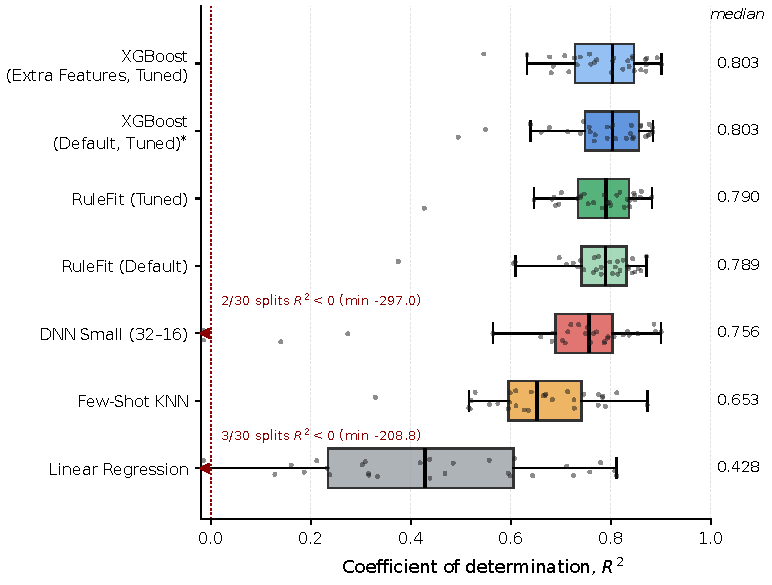
\includegraphics[width=\columnwidth]{fig01_r2_distribution.pdf}
\caption{\revmark{Distribution of held-out $R^2$ across the 30 random 70/30 train--test partitions. Boxes give the interquartile range and the median, and the superimposed dots are the 30 individual partition outcomes. The median $R^2$ is 0.803 for both XGBoost variants, 0.790 for RuleFit (Tuned), 0.789 for RuleFit (Default), 0.756 for DNN Small, 0.653 for Few-Shot KNN and 0.428 for Linear Regression. RuleFit (Tuned) has the narrowest interquartile range of the four leading models (0.102, against 0.108 and 0.117 for the two XGBoost variants), exceeds each XGBoost variant on 14 of the 30 partitions, and exceeds Few-Shot KNN on 25. Its lower quartile (0.734) almost coincides with the upper quartile of Few-Shot KNN (0.741), which is where the two distributions stop overlapping. Linear Regression and DNN Small fall below zero on 3 and 2 partitions respectively (minima $-208.8$ and $-297.0$); these outcomes are annotated rather than plotted so that the stable models remain resolvable, and they are reported numerically in Table~\ref{tab:stability}.}}
\label{fig:boxplot}
\end{figure}
\FloatBarrier


The visual overlap between the RuleFit and XGBoost distributions, together with the clearly lower KNN distribution, motivates a formal paired comparison of the repeated-split results, which is reported in Table~\ref{tab:ttest}.

%%% TABLE 4: T-TEST %%%

\begin{table}[h]
\footnotesize
\centering
\renewcommand{\arraystretch}{1.15}
\setlength{\tabcolsep}{4pt}
\caption{\revmark{Paired comparison of RuleFit (Tuned) with each comparator over the same 30 random 70/30 partitions. The layout leads with the paired mean difference, its 95\% confidence interval and Cohen's $d_z$, because effect size and interval estimates are more informative than a single $p$ value at this sample size. Only the three Few-Shot KNN comparisons survive Bonferroni correction of the 18 tests, with large effect sizes ($d_z=1.12$--$1.22$) and confidence intervals well separated from zero. Both XGBoost comparisons give negligible effect sizes ($|d_z|\le0.23$) and intervals containing zero, and the uncorrected MAE advantage over Linear Regression ($p=0.039$) does not survive correction ($p_{\mathrm{Bonf}}=0.707$).}}
\label{tab:ttest}
\begin{tabular}{@{}lrcrrr@{}}
\hline
\textbf{Comparator} & \textbf{Mean diff.} & \textbf{95\% CI} & \textbf{$d_z$} & \textbf{$p$} & \textbf{$p_{\mathrm{Bonf}}$} \\ \hline
\multicolumn{6}{@{}l}{\textit{$R^2$  (positive difference favours RuleFit)}} \\[1pt]
XGBoost (Default Features, Tuned)$^{*}$ & $-$0.013 & [$-$0.048, 0.022] & $-$0.14 & 0.769 & 1.000 \\
XGBoost (Extra Features, Tuned) & $-$0.013 & [$-$0.042, 0.016] & $-$0.17 & 0.824 & 1.000 \\
Linear Regression & +7.346 & [$-$6.924, 21.616] & +0.19 & 0.151 & 1.000 \\
RuleFit (Default) & +0.001 & [$-$0.033, 0.035] & +0.01 & 0.481 & 1.000 \\
\textbf{Few-Shot KNN} & \textbf{+0.114} & \textbf{[0.076, 0.152]} & \textbf{+1.12} & \textbf{$<$0.001} & \textbf{$<$0.001} \\
DNN Small (32--16) & +10.011 & [$-$10.285, 30.308] & +0.18 & 0.161 & 1.000 \\
\noalign{\vskip 3pt}
\multicolumn{6}{@{}l}{\textit{MAE, GPa  (negative difference favours RuleFit)}} \\[1pt]
XGBoost (Default Features, Tuned)$^{*}$ & +0.051 & [$-$0.053, 0.155] & +0.18 & 0.838 & 1.000 \\
XGBoost (Extra Features, Tuned) & +0.047 & [$-$0.044, 0.138] & +0.19 & 0.850 & 1.000 \\
Linear Regression & $-$1.492 & [$-$3.165, 0.181] & $-$0.33 & 0.039 & 0.707 \\
RuleFit (Default) & $-$0.024 & [$-$0.115, 0.066] & $-$0.10 & 0.295 & 1.000 \\
\textbf{Few-Shot KNN} & \textbf{$-$0.344} & \textbf{[$-$0.458, $-$0.230]} & \textbf{$-$1.13} & \textbf{$<$0.001} & \textbf{$<$0.001} \\
DNN Small (32--16) & $-$1.126 & [$-$3.083, 0.831] & $-$0.21 & 0.124 & 1.000 \\
\noalign{\vskip 3pt}
\multicolumn{6}{@{}l}{\textit{RMSE, GPa  (negative difference favours RuleFit)}} \\[1pt]
XGBoost (Default Features, Tuned)$^{*}$ & +0.078 & [$-$0.053, 0.209] & +0.22 & 0.884 & 1.000 \\
XGBoost (Extra Features, Tuned) & +0.070 & [$-$0.042, 0.181] & +0.23 & 0.895 & 1.000 \\
Linear Regression & $-$3.079 & [$-$7.024, 0.866] & $-$0.29 & 0.061 & 1.000 \\
RuleFit (Default) & +0.001 & [$-$0.110, 0.112] & +0.00 & 0.507 & 1.000 \\
\textbf{Few-Shot KNN} & \textbf{$-$0.438} & \textbf{[$-$0.572, $-$0.305]} & \textbf{$-$1.22} & \textbf{$<$0.001} & \textbf{$<$0.001} \\
DNN Small (32--16) & $-$2.561 & [$-$7.350, 2.228] & $-$0.20 & 0.142 & 1.000 \\
\hline
\end{tabular}
\vspace{1mm}
\scriptsize{\revmark{One-tailed paired $t$-tests of RuleFit (Tuned) against each comparator over the same 30 random 70/30 partitions ($n=30$ paired observations per test). Mean diff.\ is the paired mean of RuleFit\,$-$\,comparator. $p_{\mathrm{Bonf}}$ applies Bonferroni correction across all 18 tests. Bold rows remain significant after correction. The large mean differences and wide intervals for Linear Regression and DNN Small are a consequence of the few catastrophic partitions on which those baselines return strongly negative $R^2$ (Table~\ref{tab:stability}); their paired differences are dominated by those outliers and are not comparable in scale with the remaining rows. $^{*}$Reimplemented XGBoost baseline following the published state-of-the-art strategy of Qadir et al.~\cite{qadir2024predicting}.}}
\end{table}
\FloatBarrier

The exploratory paired tests (Table~\ref{tab:ttest}) support the same cautious interpretation. RuleFit (Tuned) does not show a statistically significant advantage over either XGBoost configuration: the $R^2$ comparison gives $t=-0.947$ and $p=0.824$ for XGBoost with engineered features and $t=-0.744$ and $p=0.769$ for the reimplemented baseline, with negligible paired effect sizes (Cohen's $d_z$ between $-0.17$ and $-0.14$) and 95\% confidence intervals of the mean $R^2$ difference that include zero ($[-0.042, 0.016]$ and $[-0.048, 0.022]$, respectively). The only clear and consistent advantage of RuleFit appears against Few-Shot KNN, for which all three metrics give large effect sizes (Cohen's $d_z=1.12$--$1.22$) with confidence intervals well separated from zero (mean $R^2$ difference $0.114$, 95\% CI $[0.076, 0.152]$); these comparisons remain significant after Bonferroni correction of all 18 tests. In contrast, the uncorrected MAE advantage over Linear Regression ($p=0.039$) does not survive correction and is not treated as a reliable difference. Because the repeated splits are overlapping, even the corrected $p$-values are used as descriptive evidence rather than as a definitive model ranking, and the interpretation relies primarily on the effect sizes and confidence intervals. The absence of a significant difference between RuleFit and the two XGBoost variants is also scientifically meaningful: it indicates that the main contribution of RuleFit is not a statistically dominant reduction in prediction error, but the conversion of a comparable predictive signal into transparent rules. For a small literature-derived ceramic dataset, this trade-off is valuable because an experimentally interpretable model with similar error to XGBoost can be more useful for hypothesis generation than a marginally more accurate black-box model.


\subsection{\revmark{Sensitivity of the Results to the Hyperparameter-Selection Step}}
\label{sec:selection}

\revmark{Reporting a model under one fixed hyperparameter configuration raises a fair question: how much of the reported performance depends on that choice? Rather than argue the point, we measured it. The entire protocol was repeated with the grid search confined to the training data alone: for every partition, the same twenty configurations were evaluated by an inner five-fold cross-validation inside the training set, the best configuration was refitted on the full training set, and the held-out partition was used exactly once, for the final score. This is a strictly leakage-free selection procedure, and it is an addition to the reported analysis rather than a replacement for it; the published protocol is retained unchanged for the reasons given in Section~2.}

\revmark{On the fixed 70/30 split, the training-only search selects \texttt{tree\_size} = 4 and \texttt{max\_rules} = 100 with an inner cross-validated $R^2$ of 0.733, and that configuration reaches $R^2 = 0.825$, MAE~=~1.506~GPa and RMSE~=~2.135~GPa on the held-out partition, against $R^2 = 0.853$, MAE~=~1.456~GPa and RMSE~=~1.958~GPa for the selected configuration re-run in the same environment. The two selection procedures differ by 0.028 in $R^2$ on this partition, which bounds how much of the fixed-split result depends on the configuration choice.}

\revmark{Across the 30 repeated partitions the two protocols are statistically indistinguishable. Selecting a configuration inside each training set gives a mean $R^2$ of $0.757 \pm 0.114$ and a mean MAE of $1.506 \pm 0.205$~GPa, whereas holding the configuration fixed gives $0.766 \pm 0.079$ and $1.466 \pm 0.214$~GPa in the same environment. The paired difference in $R^2$ is $-0.009$ with a 95\% confidence interval of $[-0.048, +0.029]$, a negligible effect size ($d_z = -0.09$) and $p = 0.62$; the training-only protocol is ahead on 14 of the 30 partitions. Two further observations explain this equivalence. The inner cross-validation selects fourteen different configurations across the thirty partitions and never selects \texttt{tree\_size} = 6 with \texttt{max\_rules} = 500, and the training-only protocol is the more variable of the two, with a standard deviation of 0.114 against 0.079. At 57 training samples, in other words, per-partition hyperparameter selection is dominated by resampling noise and buys no measurable accuracy, so fixing a single configuration in advance is not a source of detectable optimism in the repeated-partition analysis and is the more stable choice.}

\revmark{One caveat applies to these comparisons. Re-running RuleFit in the revision environment reproduces the published repeated-split mean only to within 0.003 in $R^2$ (0.766 against the reported 0.769), because the underlying tree-ensemble and coordinate-descent implementations have changed between library versions; by contrast, the XGBoost and SHAP results reproduce to four decimal places. Both arms of the comparison above were executed in the same environment, so the contrast between them is unaffected, and the package versions used for the original and the revised runs are pinned in the public repository.}

\subsection{Feature Analysis and Model Interpretability}
\label{sec:benchmark}

After evaluating predictive performance, the next objective was to determine whether the models learned relationships that are physically plausible for graphene-added Si$_3$N$_4$ ceramics. This analysis combines four complementary views: pairwise feature correlation, RuleFit linear-term importance, hierarchical feature clustering, and SHAP-based global attribution. Together, these analyses test whether the same composition, processing, and densification variables repeatedly appear as influential across independent interpretability methods.


\revmark{The feature space contains several strongly correlated groups (Fig.~\ref{fig:corr_heatmap}). Eight of the 900 feature pairs exceed $|r|=0.9$ and twenty exceed $|r|=0.8$. The two strongest are structural rather than physical: the post-sintering $\alpha$ and $\beta$ contents are exactly complementary ($r=-1.000$), and sintering energy is almost perfectly aligned with sintering time ($r=+1.000$), because in this dataset the temperature range is narrow relative to the range of holding times, so the product $T\times t$ is dominated by $t$. Sintering pressure and sintering intensity follow at $r=+0.991$ for the same reason. On the composition side, graphene content and Si$_3$N$_4$ content are strongly anticorrelated ($r=-0.879$), and additive~1 content tracks total additive content ($r=+0.911$).}

\revmark{The negative correlation between graphene content and Si$_3$N$_4$ content ($r=-0.879$) primarily reflects compositional closure in the compiled dataset: the three constituent groups sum to a fixed total, so adding graphene necessarily reduces the matrix fraction. Total additive content is anticorrelated with Si$_3$N$_4$ content for the same reason, although less strongly ($r=-0.517$), because additive levels vary over a narrower range. Although additive content can influence liquid-phase formation, densification, and grain-boundary phases, these correlations alone do not establish a mechanistic effect on hardness \cite{german2009liquid}.}

\revmark{The correlation structure in Fig.~\ref{fig:corr_heatmap} provides a direct explanation for two results in the model comparison. First, adding the eight engineered descriptors to XGBoost changes $R^2$ by only $+0.003$ on the 80/20 split (0.819 to 0.822), by $+0.018$ on the 70/30 split (0.817 to 0.835), and by only $+0.001$ in the repeated-split mean (0.782 to 0.783). These small increments are consistent with the fact that variables such as sintering energy, intensity, and dose are strongly correlated with their parent temperature, time, and pressure descriptors. The engineered representation thus reorganises existing information into interaction-oriented forms rather than adding a large amount of statistically independent information.}

\revmark{Second, the same redundancy helps explain the extreme instability of the unregularised Linear Regression model in Table~\ref{tab:stability}. Multiple descriptors constructed from the same parent variables produce a poorly conditioned feature space in which small changes in the training partition can cause large coefficient changes and extreme extrapolation. Tree-based models can use the redundant variables selectively, while RuleFit combines tree-derived thresholds with sparse regularisation. The heatmap and performance tables thus provide mutually consistent evidence: engineered descriptors can be useful as structured empirical proxies, but their value depends on a model capable of controlling or exploiting the resulting collinearity.}

\begin{figure}[h]
\centering
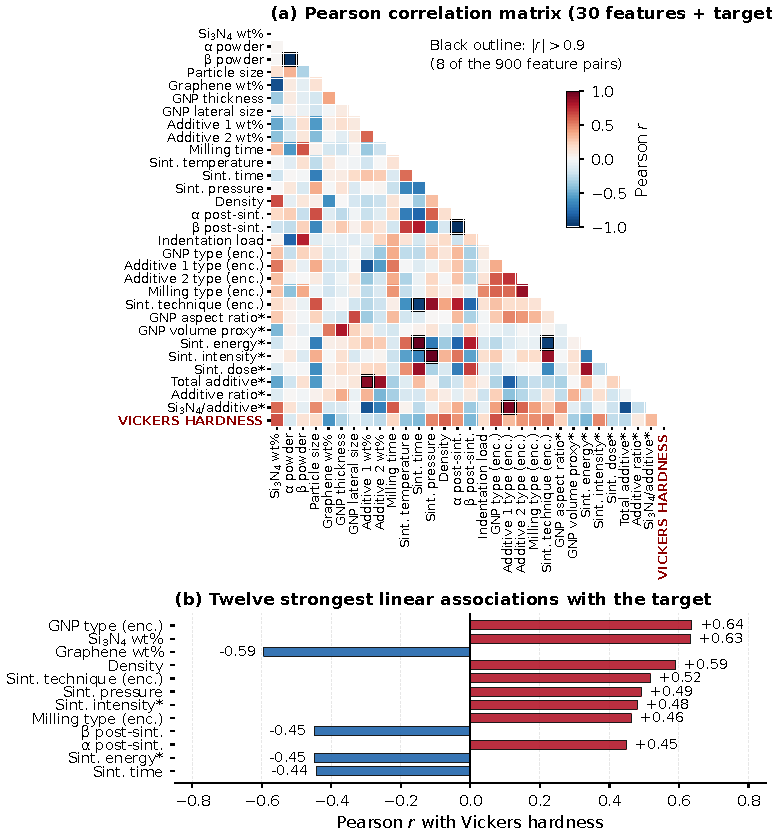
\includegraphics[width=\columnwidth]{fig02_correlation_structure.pdf}
\caption{\revmark{Correlation structure of the 30-feature input space, computed on all 82 samples. (a) Pearson correlation matrix of the original descriptors, the engineered descriptors (asterisked) and the Vickers hardness target. Cells outlined in black are the eight of the 900 feature pairs with $|r|>0.9$, listed individually in the text; twenty pairs exceed $|r|=0.8$. Coefficients are not printed inside the cells because a $31\times31$ annotated matrix cannot carry legible type within the 131~mm text block; the complete coefficient matrix is provided in the public repository. (b) The twelve strongest linear associations with hardness. The largest is only $r=+0.637$ (encoded graphene type), followed by Si$_3$N$_4$ content ($+0.634$), graphene content ($-0.594$), relative density ($+0.590$) and sintering pressure ($+0.492$); just five of the thirty descriptors exceed $|r|=0.5$, so no single variable is a dominant linear predictor of hardness.}}
\label{fig:corr_heatmap}
\end{figure}
\FloatBarrier

Graphene-related descriptors dominate the sparse linear component retained by RuleFit (Fig.~\ref{fig:feature_importance}). Graphene content carries the largest retained importance, with a value slightly above 1.0, followed by encoded graphene type at about 0.6, while density and Si$_3$N$_4$ content are smaller but still retained, with approximate importances near 0.4 and 0.2, respectively. This pattern should be interpreted together with the Boolean rules discussed below (Fig.~\ref{fig:rulefit_rules}), because RuleFit predictions use both linear terms and activated rules. The dominance of graphene content in the retained linear component suggests that graphene addition acts as a global modifier of hardness across the dataset, whereas density and Si$_3$N$_4$ content provide additional but more context-dependent corrections. This is physically plausible because graphene can influence hardness through multiple competing mechanisms, including reinforcement, crack-bridging, dispersion quality, agglomeration, and porosity formation. A sparse linear term therefore captures the average direction of this effect, while the rule component captures the conditions under which the same graphene-related variable becomes beneficial or detrimental.

\begin{figure}[h]
\centering
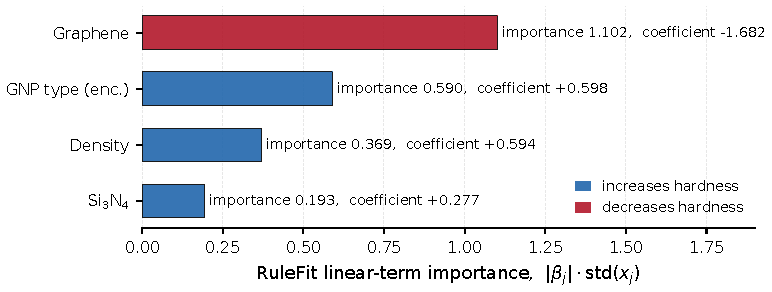
\includegraphics[width=\columnwidth]{fig03_rulefit_linear_terms.pdf}
\caption{\revmark{Retained linear terms of the tuned RuleFit model. Bar length is the linear-term importance; each annotation gives that importance together with the fitted coefficient, and the colour indicates the direction of the effect. Four linear terms survive the sparse fit: graphene content (importance 1.102, coefficient $-1.682$), encoded graphene type (0.590, $+0.598$), relative density (0.369, $+0.594$) and Si$_3$N$_4$ content (0.193, $+0.277$). Graphene content is both the strongest linear term and the only one entering with a negative sign. Among the twenty highest-importance terms of the model, these four linear terms account for 30.1\% of the total importance, so about seven tenths of the explanatory weight is carried by the Boolean rules shown in Fig.~\ref{fig:rulefit_rules}.}}
\label{fig:feature_importance}
\end{figure}
\FloatBarrier

\revmark{Hierarchical clustering provides a second representation of the correlation structure (Fig.~\ref{fig:dendrogram}). Under the distance definition $d=1-|r|$, an absolute correlation above 0.9 corresponds to a clustering distance below 0.1. Eight of the thirty merges occur below $d=0.1$, and the earliest of them reproduce exactly the redundant pairs identified in Fig.~\ref{fig:corr_heatmap}: the post-sintering $\alpha$/$\beta$ pair and the sintering-time/sintering-energy pair both merge at $d=0.0001$, the starting-powder $\alpha$/$\beta$ pair at $d=0.0049$, and the sintering-pressure/sintering-intensity pair at $d=0.0115$. These early-merging branches should not be treated as independent confirmation of a physical mechanism, because the dendrogram and heatmap are transformations of the same correlation information. Instead, they confirm that the 30-variable representation contains a small number of strongly redundant feature families.}

\revmark{At broader clustering distances, the descriptors form groups dominated by processing variables, material composition, and graphene morphology. This organisation provides a structural context for the model results: the weak performance and catastrophic partitions of the linear baseline indicate that a single additive relationship across these correlated families is insufficient, whereas the competitive $R^2$ values of RuleFit and XGBoost suggest that interactions within and between the families contain predictive information. Hardness itself joins the branch formed by relative density, Si$_3$N$_4$ content and graphene content, and it does so only at $d=0.342$; that is, its closest structural neighbours are the densification and matrix-composition descriptors rather than the post-sintering phase contents, which merge instead into the sintering-process group. The merge distance also shows that even this nearest branch is associated with hardness only at $|r|\approx0.66$, so the clustering identifies no descriptor family that would by itself determine the target, and neither the branch order nor the clustering distance establishes a causal mechanism. The dendrogram therefore supports a multivariable and interaction-dependent interpretation of hardness while remaining an exploratory description of feature organisation.}

\begin{figure}[h]
\centering
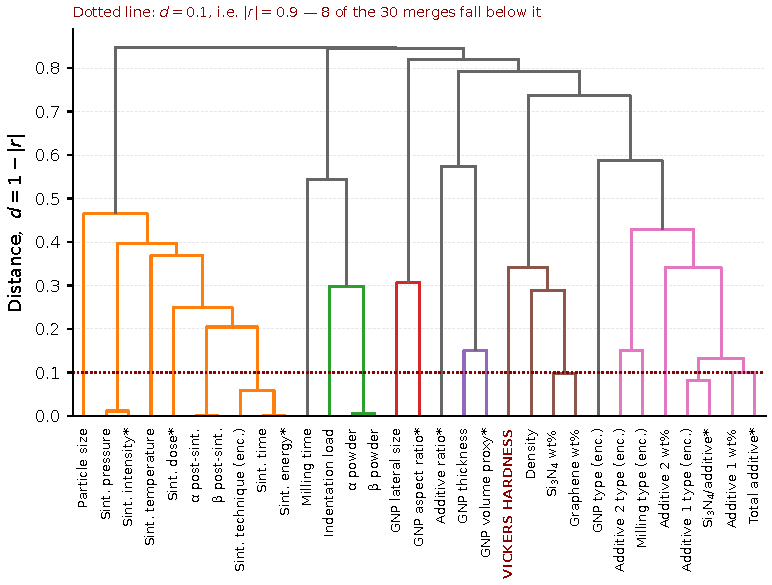
\includegraphics[width=\columnwidth]{fig04_dendrogram.pdf}
\caption{\revmark{Hierarchical clustering of the 30 input descriptors together with the Vickers hardness target, computed on the training partition of the fixed 70/30 split. Average linkage is applied to the correlation-based distance $d=1-|r|$; average linkage is used because the distance matrix is supplied rather than Euclidean, so a variance-minimising criterion would not be appropriate. Eight of the thirty merges occur below the dotted line at $d=0.1$, that is at $|r|>0.9$. The earliest merges are the post-sintering $\alpha$/$\beta$ pair and the sintering-time/sintering-energy pair (both at $d=0.0001$), the starting-powder $\alpha$/$\beta$ pair ($d=0.0049$) and the sintering-pressure/sintering-intensity pair ($d=0.0115$), which is the same redundancy structure identified in Fig.~\ref{fig:corr_heatmap}. The target merges with the branch containing relative density, Si$_3$N$_4$ content and graphene content at $d=0.342$, corresponding to $|r|\approx0.66$ for that branch; no descriptor joins hardness at a distance that would indicate a single dominant driver. The broader groups are consistent with three physical families: sintering process variables, material composition variables, and graphene morphology descriptors.}}
\label{fig:dendrogram}
\end{figure}
\FloatBarrier

\revmark{SHAP attribution provides an additional check on the variables identified by RuleFit (Fig.~\ref{fig:shap_summary}). The highest-ranked features include sintering pressure, encoded graphene type, Si$_3$N$_4$ content, graphene content, and density, in good agreement with the variables retained by the sparse RuleFit linear component (Fig.~\ref{fig:feature_importance}). SHAP additionally identifies sintering pressure as a major contributor, which is physically reasonable because pressure-assisted densification directly affects hardness. These convergent observations support the interpretation that the model is not relying on a single isolated variable. The partial agreement between SHAP and RuleFit is especially important because the two explanations are obtained from different model families. SHAP reflects the attribution structure of the interpretability XGBoost model, whereas RuleFit retains only a sparse subset of linear terms and threshold rules. Their convergence on graphene type/content, pressure, density, and Si$_3$N$_4$ content suggests that these variables are robust predictors rather than artefacts of a single algorithm. At the same time, the higher SHAP importance of sintering pressure compared with its weaker appearance in the RuleFit linear terms indicates that pressure may act mainly through threshold-like or interaction-dependent effects rather than as a simple monotonic linear contributor.}

The comparison between the RuleFit and SHAP explanations reveals both convergence and model-specific reliance. Across the 25 samples in the fixed 70/30 test set, the five leading SHAP variables include sintering pressure, encoded graphene type, Si$_3$N$_4$ content, graphene content, and density. RuleFit retains a related but differently weighted linear structure: graphene content has an importance slightly above 1.0, followed by encoded graphene type at approximately 0.6, density near 0.4, and Si$_3$N$_4$ content near 0.2. The absence of a similarly dominant linear pressure term in RuleFit, despite the high SHAP ranking of pressure, is consistent with pressure entering RuleFit mainly through Boolean interactions rather than through a global monotonic contribution.

This distinction is also reflected in the pre-synthesis ablation. Removing density and the $\alpha$/$\beta$ phase descriptors reduces the mean RuleFit $R^2$ by only 0.007, from $0.769$ to $0.762$, whereas the mean XGBoost $R^2$ decreases by 0.062, from $0.783$ to $0.721$. Thus, the high SHAP ranking of post-sintering information is accompanied by a larger predictive dependence on those variables in XGBoost, while RuleFit preserves more of its mean accuracy through composition- and processing-based rules. RuleFit variability nevertheless increases from 0.089 to 0.112 after the ablation, showing that the removed descriptors contribute to stability even when their effect on mean performance is small. These results reinforce that feature attribution is conditional on the model architecture and should not be interpreted as a model-independent ranking of physical causation. The observed graphene-, pressure-, and density-related contributions remain associations that may also encode dispersion quality, porosity, processing route, and source-specific experimental conditions \cite{ramirez2014extraordinary,qadir2024predicting}.
\begin{figure}[h]
\centering
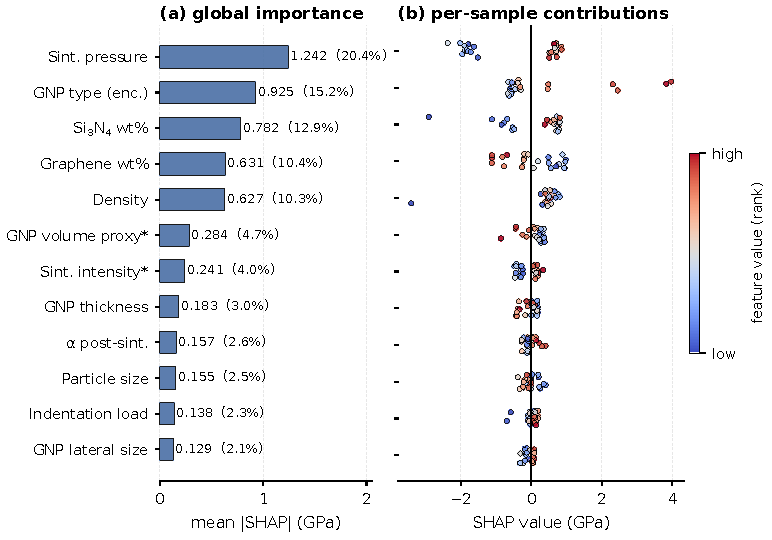
\includegraphics[width=\columnwidth]{fig05_shap_summary.pdf}
\caption{\revmark{Global SHAP attribution for the interpretability XGBoost model on the 25 held-out samples of the fixed 70/30 split. (a) Mean absolute SHAP value per descriptor, annotated with its share of the total attribution: sintering pressure 1.242~GPa (20.4\%), encoded graphene type 0.925~GPa (15.2\%), Si$_3$N$_4$ content 0.782~GPa (12.9\%), graphene content 0.631~GPa (10.4\%) and relative density 0.627~GPa (10.3\%). The three leading descriptors carry 48.5\% of the attribution and the five leading ones 69.2\%. (b) The individual per-sample SHAP values behind those means, coloured by the rank of the corresponding feature value. Every leading descriptor takes both signs across the test set --- sintering pressure spans $-2.375$ to $+0.857$~GPa and relative density $-3.406$ to $+0.808$~GPa --- so none of them acts in one direction independently of the surrounding processing context. The ranking is broadly consistent with the RuleFit interpretation in Figs.~\ref{fig:feature_importance} and~\ref{fig:rulefit_rules}.}}
\label{fig:shap_summary}
\end{figure}
\FloatBarrier

The strongest retained RuleFit terms and Boolean rules are summarised in Fig.~\ref{fig:rulefit_rules}. The largest linear term is graphene content, with coefficient $-1.682$ and support of 1.00, indicating a global negative contribution when all samples are considered. The strongest positive rule combines load, encoded graphene type, and density, with coefficient $+1.626$ and support of 0.43, whereas a high-graphene and low-sintering-intensity rule contributes negatively, with coefficient $-2.133$ and support of 0.11. These values make the plot useful not only as an importance ranking, but also as a compact rule-level explanation of the model. Because the practical transparency of the rules depends on their exact threshold values, the complete set of retained rules, including all thresholds, coefficients, and support values, is provided in machine-readable form in the public repository (\texttt{rulefit\_top\_rules.csv}); the figure compresses long conjunctive rules only for display purposes. The negative graphene-content coefficient indicates that, averaged over all samples, increasing graphene content tends to reduce predicted hardness. This should not be interpreted as evidence that graphene is intrinsically harmful in Si$_3$N$_4$ ceramics; rather, it suggests that in the available dataset, high graphene loading is often associated with conditions that reduce hardness, such as agglomeration, incomplete densification, or reduced effective ceramic matrix continuity. Conversely, the strongest positive Boolean rule combines load, encoded graphene type, and density, indicating that favourable hardness predictions emerge when graphene-related information is accompanied by sufficient densification. The high-graphene/low-sintering-intensity negative rule is particularly informative because it provides an experimentally testable hypothesis: graphene-rich formulations may require sufficiently strong thermal--mechanical sintering conditions to avoid a hardness penalty.

This rule is consistent with a processing--composition interaction in which the association of graphene-related descriptors with hardness depends on densification-related variables. Because the dataset does not contain direct measurements of interfacial pull-out, crack bridging, or related micromechanical mechanisms, the rule should not be assigned to a specific toughening mechanism without targeted microstructural validation.

\begin{figure}[h]
\centering
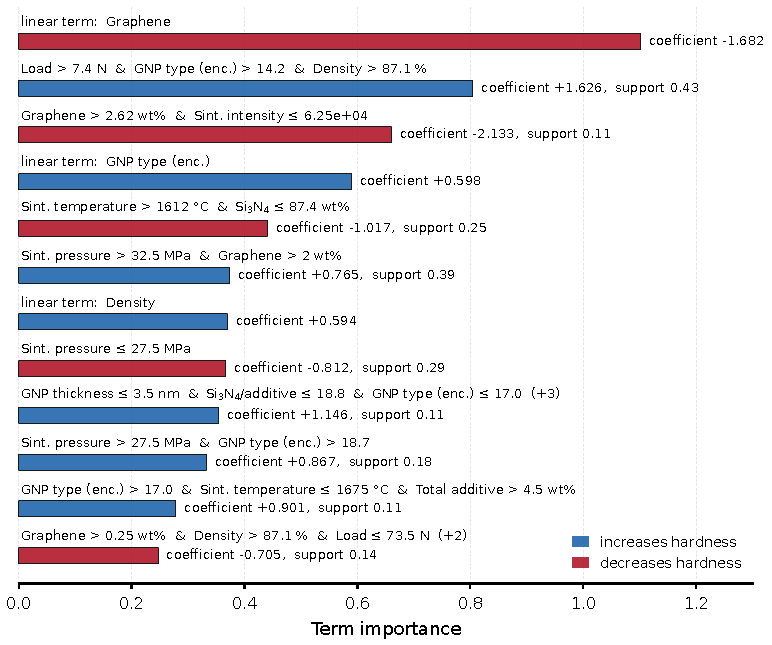
\includegraphics[width=\columnwidth]{fig06_rulefit_rules.pdf}
\caption{\revmark{The twelve highest-importance terms of the tuned RuleFit model. Bar length is the term importance; each annotation gives the fitted coefficient and, for Boolean rules, the support. RuleFit is fitted on standardised training data, so the thresholds stored with the model are $z$-scores of the training partition; they are inverted here to physical units so that each rule can be read directly as a processing condition. The strongest single term is the linear graphene-content term (coefficient $-1.682$). The strongest positive rule (coefficient $+1.626$, support 0.43) requires an indentation load above 7.4~N, an encoded graphene type above 14.2 and a relative density above 87.1\%. The strongest negative rule (coefficient $-2.133$, support 0.11) combines a graphene content above 2.62~wt.\% with a sintering intensity at or below $6.25\times10^{4}$, that is, a graphene-rich composition processed under a low temperature--pressure product. Rule supports range from 0.07 to 0.43 with a mean of 0.21, so the largest coefficients belong to rules active for a minority of the training samples. Conjunctions longer than three conditions are truncated with the number of omitted conditions in parentheses; the complete rule set, in both standardised and physical units, is in the public repository (\texttt{rulefit\_rules\_physical\_units.csv}).}}
\label{fig:rulefit_rules}
\end{figure}
\FloatBarrier

\revmark{Taken together, Figs.~\ref{fig:corr_heatmap}--\ref{fig:rulefit_rules} indicate that the predictive signal is not concentrated in a single isolated descriptor. Instead, hardness is associated with a coupled feature structure involving graphene addition, Si$_3$N$_4$ content, relative density, and sintering conditions. The heatmap and dendrogram show that several engineered descriptors are strongly linked to their parent processing variables, while the RuleFit and SHAP analyses identify overlapping but not identical influential features. This partial agreement is expected because RuleFit emphasises sparse linear terms and Boolean thresholds, whereas SHAP summarises the contribution structure of the interpretability XGBoost model. The convergence of these independent explanations around graphene-related variables, sintering pressure, density, and Si$_3$N$_4$ content strengthens the interpretation that the model is capturing physically meaningful processing--structure--property patterns rather than relying solely on numerical artefacts. In ceramic terms, this pattern is consistent with the expected competition between reinforcement and densification: graphene-related descriptors may reflect beneficial interfacial or toughening-related effects at suitable additions, but excessive graphene can also reduce hardness by promoting agglomeration, porosity, or incomplete load transfer. Similarly, sintering pressure and relative density are expected to increase hardness by improving particle rearrangement, reducing residual porosity, and supporting a more compact Si$_3$N$_4$ matrix. The negative association of total additive content with Si$_3$N$_4$ content should therefore be interpreted as part of a compositional balance rather than as an isolated causal effect.}

The extracted thresholds for sintering time and temperature may reflect nonlinear associations related to liquid-phase sintering and phase evolution, but they should not be interpreted as direct kinetic constants or mechanistic transition points \cite{german2009liquid}. Similarly, the contributions of graphene type and thickness are consistent with morphology-dependent effects reported for ceramic--graphene composites, while the present dataset does not directly resolve dispersion, crack deflection, pull-out, grain coarsening, or stress-concentration mechanisms \cite{miranzo2017bulk,ramirez2014extraordinary}. The SHAP results should therefore be interpreted as context-dependent feature associations rather than direct evidence of specific microstructural processes.


\subsection{Data Structure Visualisation}
\label{sec:datastructure}

\revmark{The two-dimensional projections in Fig.~\ref{fig:pca_tsne} provide a geometric context for the model-performance results. PC1 and PC2 explain 28.8\% and 17.5\% of the variance, respectively, so the PCA panel represents 46.3\% of the total feature variance and necessarily omits the remaining 53.7\%. The projection is a weak summary of the feature space: six components are needed to reach 80\% of the variance and eight to reach 90\%, so the thirty descriptors do not collapse onto a low-dimensional manifold. The $t$-SNE projection, generated with perplexity 15, suggests partial local separation between the fifteen samples below 10~GPa and the seven above 20~GPa, but the sixty intermediate-hardness samples overlap extensively, indicating that hardness is not organised into a small number of compact two-dimensional clusters.}

This overlap is consistent with the relative weakness of the distance-based Few-Shot KNN model, which reaches a mean $R^2$ of $0.655 \pm 0.113$, compared with $0.769 \pm 0.089$ for RuleFit and approximately 0.782--0.783 for the XGBoost variants. A nearest-neighbour model assumes that samples close under the standardised Euclidean metric have similar targets, whereas the PCA and $t$-SNE projections indicate that samples with different hardness values can occupy overlapping regions. RuleFit and XGBoost can instead separate such samples through combinations and thresholds involving graphene type, pressure, density, additive balance, and phase content. This agreement between the projection structure and the model comparison does not prove that overlap causes the KNN performance gap, particularly because $t$-SNE does not preserve global distances; however, it supports the interpretation that hardness depends on high-dimensional, context-specific relationships rather than on simple local proximity. It also explains why sample-level explanations remain necessary even after global feature ranking.

\begin{figure}[h]
\centering
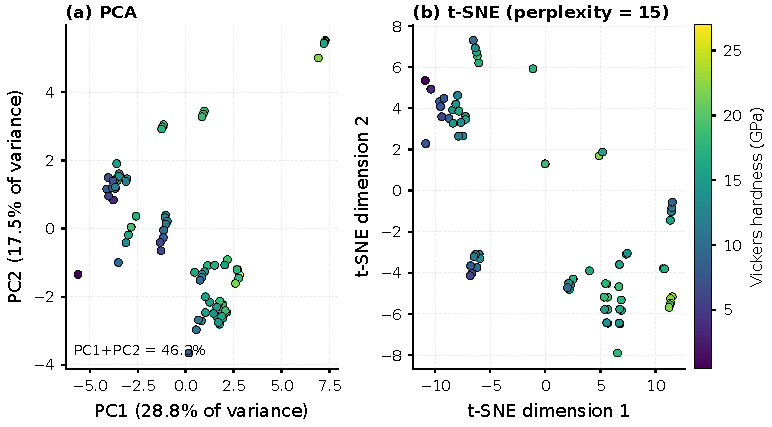
\includegraphics[width=\columnwidth]{fig07_pca_tsne.pdf}
\caption{\revmark{Two-dimensional projections of the 30-feature dataset, each point being one of the 82 samples coloured by its measured Vickers hardness. (a) PCA of the standardised feature matrix: PC1 explains 28.8\% and PC2 17.5\% of the variance, so the panel represents 46.3\% of the total variance and omits the remaining 53.7\%. Six components are required to reach 80\% of the variance and eight to reach 90\%, which indicates that the feature space is not effectively two-dimensional. (b) $t$-SNE projection with perplexity~=~15. Fifteen samples lie below 10~GPa and seven above 20~GPa, while the remaining sixty occupy the intermediate range; the low- and high-hardness samples show partial local separation, but the intermediate majority overlaps extensively, so the projections do not resolve discrete hardness regimes. Both panels are computed from the same target-encoded 30-feature matrix that is used for model training.}}
\label{fig:pca_tsne}
\end{figure}
\FloatBarrier





\subsection{Case Study: Interpretability Analysis of RuleFit Predictions}
\label{sec:casestudy}

\revmark{To complement the global analyses, five test samples were selected to represent distinct local explanation regimes rather than to form a statistically representative benchmark. RuleFit errors are 0.044 and 0.138~GPa for the two highly accurate cases P1 and P2, 0.832 and 0.846~GPa for the intermediate cases P3 and P4, and 4.459~GPa for the high-hardness boundary case P5 (Table~\ref{tab:case_overview}). Across these deliberately stratified cases, the mean absolute RuleFit error is 1.264~GPa; however, this value falls to 0.465~GPa when P5 is excluded, and P5 alone accounts for approximately 70.6\% of the total absolute RuleFit error across the five samples. The selected-case error is strongly concentrated in the upper-boundary observation rather than being distributed uniformly.}

\revmark{The XGBoost errors show a different local pattern. Its selected-case mean absolute error is 1.930~GPa, with substantial contributions from both P1 (2.709~GPa) and P5 (5.087~GPa), despite its strong aggregate performance in Tables~\ref{tab:80_20}--\ref{tab:stability}. These values must not be interpreted as a five-sample model ranking because the cases were intentionally selected by error regime. Instead, they demonstrate that comparable global metrics can arise from different local failure patterns: RuleFit is highly accurate for P1 but misses the upper target boundary at P5, whereas XGBoost has difficulty with both the graphene-rich low-pressure case and the high-hardness boundary case. Figure~\ref{fig:shap_waterfall} serves to explain model-specific local behaviour that is not visible from global MAE or $R^2$ alone. Complementary LIME explanations were generated with 1\,000 perturbation samples.}

\begin{table}[h]
\footnotesize
\centering
\renewcommand{\arraystretch}{1.4}
\caption{Selected test samples used for local interpretability analysis. The table reports measured Vickers hardness, RuleFit prediction, XGBoost prediction, absolute RuleFit error, and qualitative error category. The error categories refer to the RuleFit predictions only; the XGBoost predictions are listed for comparison and can deviate substantially for individual samples (e.g., P1). P1 and P2 are very accurate RuleFit cases with errors of 0.044 and 0.138~GPa, while P5 is the most challenging case with a 4.459~GPa RuleFit error.}
\label{tab:case_overview}
\begin{tabular}{cccccc}
\hline
\textbf{Point} & \textbf{True (GPa)} & \textbf{RF Pred.} & \textbf{XGB Pred.} & \textbf{RF Error} & \textbf{Category} \\ \hline
P1 & 6.5  & 6.544  & 9.209  & 0.044 & Very accurate ($<$0.2~GPa) \\
P2 & 18.3 & 18.438 & 18.406 & 0.138 & Very accurate ($<$0.2~GPa) \\
P3 & 13.3 & 14.132 & 14.432 & 0.832 & Moderate (0.8--0.9~GPa) \\
P4 & 15.5 & 14.654 & 14.882 & 0.846 & Moderate (0.8--0.9~GPa) \\
P5 & 27.0 & 22.541 & 21.913 & 4.459 & Challenging ($>$3.5~GPa) \\
\hline
\end{tabular}
\end{table}
\FloatBarrier

\paragraph{Point P1 (True: 6.5~GPa, RF: 6.544~GPa, XGB: 9.209~GPa).}
This low-hardness sample combines high graphene content (8.0~wt.\%) with low sintering pressure (25~MPa). RuleFit activates negative rules associated with excess graphene and insufficient sintering intensity, bringing the prediction close to the measured value. SHAP and LIME point to the same local pattern: low pressure and graphene-related descriptors move the prediction downward. The case therefore provides a compact example of how the activated rules make a low-hardness prediction easier to inspect in terms of processing and composition conditions.

P1 also exposes an instructive discrepancy between global and local model behaviour. Although XGBoost achieves strong aggregate error metrics (MAE between approximately 1.25~GPa on the fixed 80/20 split and 1.60~GPa on the fixed 70/30 split), its prediction for this particular sample (9.209~GPa against a measured 6.5~GPa) deviates by about 2.7~GPa, well above its typical error, whereas RuleFit predicts the same sample almost exactly. This behaviour is consistent with the position of P1 in the feature space: samples combining very high graphene loading with low sintering pressure are sparsely represented in the dataset, and in such sparsely populated regions a boosted ensemble tends to regress towards the bulk of the training distribution, pulling the prediction upward towards mid-range hardness values. RuleFit, in contrast, retains an explicit negative rule for the high-graphene/low-sintering-intensity regime, so its prediction follows the threshold behaviour rather than the global trend. The example illustrates that strong global metrics do not guarantee uniform local reliability, particularly near the boundaries of a small dataset, and that sample-level explanations are needed precisely for this reason. It should also be noted that the SHAP decomposition discussed below explains the XGBoost prediction of 9.209~GPa, not the RuleFit prediction to which the ``very accurate'' category in Table~\ref{tab:case_overview} refers.

\paragraph{Point P2 (True: 18.3~GPa, RF: 18.438~GPa, XGB: 18.406~GPa).}
This high-hardness sample contains no graphene and combines high sintering pressure (50~MPa) with high relative density. RuleFit activates positive rules linked to pressure and density, while SHAP and LIME also rank densification-related variables among the main positive contributors. The agreement across methods indicates that this prediction is mainly driven by pressure-assisted densification rather than by a graphene-reinforcement effect.

\paragraph{Point P3 (True: 13.3~GPa, RF: 14.132~GPa, XGB: 14.432~GPa).}
This sample has no graphene and is processed at very low sintering pressure (20~MPa). No extracted RuleFit rule is activated, so the prediction is mainly governed by the linear component and is moderately overestimated. SHAP and LIME both identify low sintering pressure as the dominant downward factor. This behaviour suggests that very low-pressure conditions remain difficult for both RuleFit and XGBoost when few comparable samples are available.

\paragraph{Point P4 (True: 15.5~GPa, RF: 14.654~GPa, XGB: 14.882~GPa).}
This intermediate case contains moderate graphene addition together with high density and high sintering pressure. RuleFit activates rules with opposite signs: a positive pressure-related rule and a negative rule involving density, graphene type, and load. The partial cancellation of these terms explains the modest underestimation. SHAP and LIME show a similar balance between positive pressure/composition effects and negative graphene-related effects.

\paragraph{Point P5 (True: 27.0~GPa, RF: 22.541~GPa, XGB: 21.913~GPa).}
This sample is the most difficult case in the test set. Both RuleFit and XGBoost underestimate its very high measured hardness, despite high density and high sintering pressure. The explanation methods point to graphene type and pressure as favourable factors, but their combined contribution is still insufficient to reach the measured 27.0~GPa. From an experimental-design perspective, P5 is particularly informative because it identifies the type of sample for which the current model is least reliable: a high-hardness composition located near the upper boundary of the available target range. Such cases are valuable because they can guide future validation experiments. If additional samples with similar graphene type, high density, and high sintering pressure confirm hardness values close to 27~GPa, the model would require retraining with better representation of this high-performance region. Conversely, if new measurements fall closer to the model prediction, the apparent outlier behaviour of P5 may reflect source-specific experimental variation or measurement heterogeneity.

The underestimation of P5 is more conservatively interpreted as a boundary-of-domain error: its measured hardness lies at the upper end of the target distribution, where few comparable training samples are available. The available data do not establish whether this value represents a reproducible high-performance regime, a source-specific measurement effect, or an unusual experimental condition. Additional measurements under comparable processing conditions are therefore required before assigning a physical explanation to this residual.

\revmark{The SHAP waterfall explanations in Fig.~\ref{fig:shap_waterfall} decompose the interpretability XGBoost predictions relative to a common base value of 14.933~GPa. For P1, the final prediction of 9.209~GPa represents a total downward shift of 5.724~GPa. Sintering pressure ($-1.896$~GPa) and graphene content ($-1.116$~GPa) jointly account for $-3.012$~GPa of this shift, while the remaining features contribute a net additional reduction of approximately 2.712~GPa. The low prediction is not produced by one dominant descriptor alone, but by a broader set of mutually reinforcing negative contributions.}

\revmark{For P2, the prediction of 18.406~GPa is 3.473~GPa above the base value. Density ($+0.778$~GPa), Si$_3$N$_4$ content ($+0.703$~GPa), and sintering pressure ($+0.688$~GPa) contribute a combined $+2.169$~GPa, corresponding to approximately 62.5\% of the total upward shift. This concentration of positive attribution in three densification- and matrix-related variables is consistent with the global SHAP ranking in Fig.~\ref{fig:shap_summary}. P3 exhibits a more compensatory pattern. The positive contributions from graphene content ($+0.946$~GPa), Si$_3$N$_4$ content ($+0.650$~GPa) and density ($+0.560$~GPa) total $+2.156$~GPa, which exceeds the $-1.785$~GPa sintering-pressure contribution by 0.371~GPa. The final prediction nevertheless remains 0.448~GPa below the base value, because the encoded graphene type ($-0.577$~GPa), sintering intensity ($-0.295$~GPa) and the pooled remaining descriptors ($+0.053$~GPa) together offset that surplus.}

The three decompositions therefore illustrate distinct local structures: cumulative negative attribution for P1, concentrated positive densification-related attribution for P2, and cancellation among competing effects for P3. This cross-sample comparison explains why a globally important feature cannot be assigned one universal direction of effect and why the SHAP summary, RuleFit rules, and sample-level explanations must be interpreted together.

\begin{figure}[h]
\centering
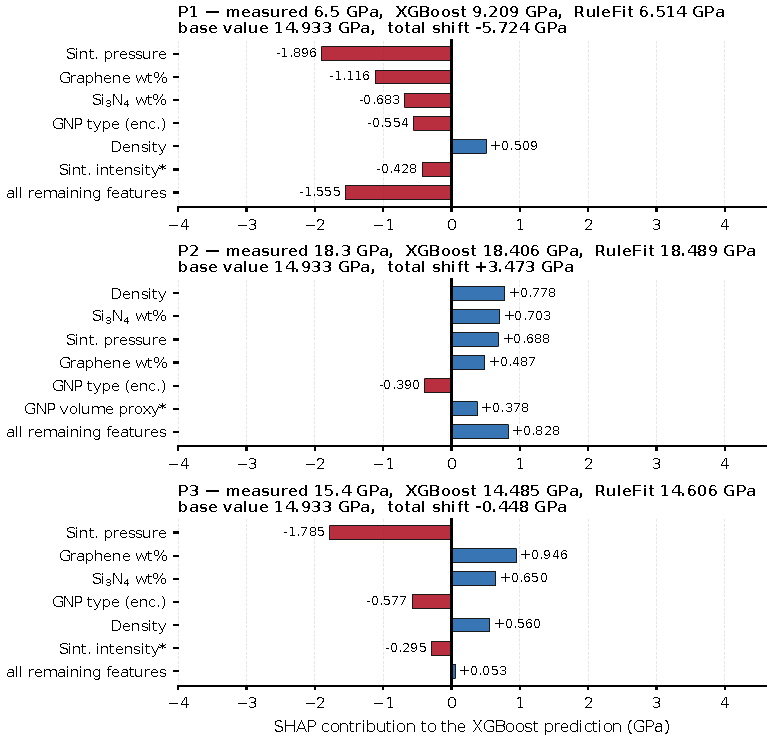
\includegraphics[width=\columnwidth]{fig08_shap_local.pdf}
\caption{\revmark{Local SHAP decompositions for test samples P1, P2 and P3. All three panels explain the interpretability XGBoost model, whose common base value is 14.933~GPa; the accuracy categories in Table~\ref{tab:case_overview} instead refer to the RuleFit predictions, which is why P1 is listed as a very accurate RuleFit case (RuleFit 6.514~GPa against a measured 6.5~GPa) even though the XGBoost prediction for the same sample is 9.209~GPa. Each panel shows the six largest individual contributions and pools the remaining twenty-four descriptors into a single bar, so the plotted terms sum exactly to the stated total shift. The three samples illustrate three distinct local structures: cumulative negative attribution for P1 ($-5.724$~GPa overall, led by sintering pressure and graphene content), concentrated densification-related positive attribution for P2 ($+3.473$~GPa, led by density, Si$_3$N$_4$ content and pressure), and near-cancellation for P3, where a $-1.785$~GPa pressure term is offset by positive graphene, matrix and density terms to leave a net shift of only $-0.448$~GPa. The individual values are given in the text.}}
\label{fig:shap_waterfall}
\end{figure}
\FloatBarrier


\subsection{Limitations, Future Directions, and Experimental Validation}

Despite its competitive predictive performance and transparent rule-based structure,
the present framework should be interpreted within the methodological constraints
inherent to literature-derived, small-sample ceramic datasets. These constraints do
not undermine the central finding that interpretable rule-based learning can approach the performance of strong black-box baselines; rather, they clarify the conditions under which the reported predictions, feature attributions, and extracted rules can be considered reliable. Three limitations are particularly important for interpreting the present results and for guiding future experimental and computational work.

\revmark{Several of these constraints were accepted deliberately rather than overlooked, and the reasoning is stated here so that the trade-off is explicit. The study is designed as a head-to-head comparison with the published XGBoost workflow of Qadir et al.~\cite{qadir2024predicting} on the same 82-sample dataset. A comparison of that kind is informative only while both methods are evaluated under identical conditions, so the dataset, the feature construction, the split sizes and the evaluation protocol of the reference study were preserved. Changing any of them --- including changes that would be methodologically preferable when a method is assessed on its own --- would alter the conditions on one side of the comparison only and would bias the result against the reference method. This is why no additional samples were collected: a larger dataset would improve the model but would make the difference between the two workflows uninterpretable, because it would confound the change of method with a change of data. The consequences of the small sample size were addressed instead by statistical means that leave the protocol intact, namely repeated evaluation over 30 random partitions of the same data, effect sizes and confidence intervals alongside multiplicity-corrected $p$ values (Tables~\ref{tab:stability} and~\ref{tab:ttest}), a leave-one-reference-out analysis of source heterogeneity, and the leakage-free re-analysis of Section~\ref{sec:selection}. The complete dataset, feature-generation code, model-training scripts, evaluation scripts and random seeds are public, so every choice described here can be inspected and re-executed independently.}

First, the dataset remains small and literature-derived. Although the 82-sample dataset is valuable because it aggregates characterised graphene-added Si$_3$N$_4$ ceramics experimentally, its size limits the statistical power of model comparison and increases sensitivity to train--test partitioning. This limitation is partly addressed in the present work through fixed 80/20 and 70/30 splits together with a 30-replicate random-split stability analysis. Nevertheless, future work should expand the dataset through systematic experimental campaigns in which graphene type, graphene content, sintering pressure, sintering temperature, holding time, additives, density, and phase composition are varied under controlled conditions. A larger and more balanced dataset would enable more reliable external validation, uncertainty quantification, and stricter benchmarking of interpretable and black-box models.

Second, the dataset was compiled from sixteen literature sources, introducing source-dependent heterogeneity in powder preparation, milling, sintering equipment, indentation conditions, reporting conventions, and measurement calibration. Random splitting can place observations from the same source in both the training and test sets, so excluding the source label does not eliminate implicit inter-batch information encoded through the measured descriptors.

The magnitude of this effect is quantified by the leave-one-reference-out analysis. Relative to the repeated random-split result, RuleFit $R^2$ decreases from 0.769 to 0.39, an absolute reduction of 0.379 or approximately 49\%, while MAE increases from 1.467 to 3.01~GPa, corresponding to an increase of approximately 105\%. For XGBoost with engineered features, $R^2$ decreases from 0.783 to 0.49, an absolute reduction of 0.293 or approximately 37\%, and MAE increases from 1.420 to 2.80~GPa, an increase of approximately 97\%. The XGBoost--RuleFit difference consequently expands from only 0.014 in mean random-split $R^2$ to 0.10 under source-level exclusion, while the LORO MAE favours XGBoost by 0.21~GPa. Thus, the near-equivalence of the models under random splitting does not fully transfer to unseen-source evaluation.

Per-source MAE values range from approximately 0.9 to 6.6~GPa, representing more than a sevenfold difference among held-out sources. This variation indicates that some literature domains are well represented by the remaining studies, whereas others occupy poorly covered processing or measurement regimes. Importantly, the result also qualifies the interpretation of the RuleFit rules: transparent thresholds can still be conditioned by source-specific ranges even when the source identifier is excluded. Random-split performance should therefore be interpreted as interpolation within the compiled literature domain, while LORO provides the more relevant estimate for transfer to new laboratories or processing routes. Future work should combine source-aware validation with harmonised multi-laboratory measurements and explicit uncertainty estimates for out-of-domain predictions.

Third, the full feature set contains post-sintering descriptors, particularly relative density and $\alpha$/$\beta$-Si$_3$N$_4$ phase content. Their use defines a process--structure--property model suitable for post-synthesis interpretation or quality monitoring, rather than a purely pre-synthesis composition--process--property model. This distinction is quantitatively examined by removing the three post-sintering descriptors and repeating the 30-split analysis with 27 features.

\revmark{The two model families respond differently to this ablation. RuleFit mean $R^2$ decreases by only 0.007, from $0.769$ to $0.762$, corresponding to a relative reduction of approximately 0.9\%, and MAE increases by only 0.023~GPa, from 1.467 to approximately 1.49~GPa. However, its $R^2$ standard deviation increases from 0.089 to 0.112, an increase of approximately 26\%. RuleFit retains almost the same average accuracy without the post-sintering variables, but its predictions become more partition-sensitive. XGBoost shows a stronger dependence: mean $R^2$ decreases by 0.062, from $0.783$ to $0.721$, a relative reduction of approximately 7.9\%, MAE increases from 1.420 to 1.56~GPa, and the $R^2$ standard deviation increases from 0.084 to 0.153, an increase of approximately 82\%.}

These changes provide an important cross-check of the interpretability analysis. Density and phase-related information appears prominently in the XGBoost SHAP structure, and removing it produces both a larger accuracy loss and a larger increase in variance for XGBoost. RuleFit relies more heavily on composition--processing thresholds that partially substitute for the missing post-sintering information, although with reduced stability. A pre-synthesis RuleFit variant is therefore feasible as a hypothesis-screening model, but it should not be interpreted as having equivalent reliability to the full-feature model. A complete prospective design framework would require external validation and, where possible, coupled models that predict density and phase composition from controllable processing variables before hardness is estimated.

Overall, these limitations do not undermine the main conclusion that interpretable
rule-based learning can reach the performance range of strong black-box baselines
on small ceramic datasets. Instead, they define the next steps required to move from
retrospective literature-based modelling toward experimentally validated ceramic
informatics. In particular, future studies should prioritise targeted fabrication of
samples in the high-hardness regions suggested by the model, independent testing on
newly produced graphene-added Si$_3$N$_4$ ceramics, and prospective validation of
the most physically meaningful RuleFit rules. Such validation would determine whether the identified relationships among graphene addition, sintering pressure, density, Si$_3$N$_4$ content, and hardness can be used not only to explain existing data, but also to guide the design of improved ceramic composites.


\section{Conclusion}

This study presented an interpretable machine learning framework for predicting the Vickers hardness of graphene-added Si$_3$N$_4$ ceramics using a dataset of 82 experimentally characterised samples. A tuned RuleFit model was evaluated alongside multiple comparator configurations, including XGBoost with original and engineered features, regularised and unregularised linear baselines, Few-Shot KNN, a default RuleFit configuration, and a small deep neural network. Performance was assessed using fixed 80/20 and 70/30 train--test splits and a 30-replicate random-split stability analysis.

On the 70/30 fixed split, RuleFit (Tuned) achieved the highest performance (R$^2$ = 0.854, RMSE~$= 1.955$~GPa, MAE~$= 1.477$~GPa), surpassing both XGBoost variants (R$^2$ = 0.817--0.835) and DNN Small (R$^2$ = 0.836). Across 30 random splits, RuleFit demonstrated stable performance (R$^2$ = $0.769 \pm 0.089$), comparable to XGBoost (R$^2$ = $0.782 \pm 0.096$). Exploratory one-tailed paired $t$-tests showed a consistent advantage of RuleFit only over Few-Shot KNN, with large effect sizes (Cohen's $d_z = 1.12$--$1.22$) that remain significant after Bonferroni correction, while the differences with XGBoost and DNN are small in effect size and not statistically distinguishable. Linear Regression and DNN exhibited high instability (mean R$^2 < 0$, i.e., worse than mean prediction on some partitions) attributable to feature collinearity and overparameterisation at this dataset size. A leave-one-reference-out validation further showed that cross-source generalisation is substantially harder than random-split evaluation (pooled R$^2$ of 0.39 for RuleFit and 0.49 for XGBoost), whereas removing the post-sintering descriptors reduced random-split performance only moderately (RuleFit R$^2 = 0.762 \pm 0.112$), indicating that a pre-synthesis variant of the framework is feasible.

Feature importance analysis and hierarchical clustering identified three physically meaningful feature families: sintering process parameters, material composition, and graphene morphology descriptors. Graphene content/type, sintering pressure, Si$_3$N$_4$ content, and relative density emerged as recurring predictors across RuleFit and SHAP analyses, aligning with established ceramic processing--property relationships.

The five-sample case study shows how RuleFit rule activations can be used to inspect individual predictions rather than only reporting global accuracy. In particular, the activated rules highlight two recurring effects: the penalty associated with relatively high graphene content under insufficient sintering intensity, and the beneficial role of high sintering pressure in dense samples. SHAP and LIME provide qualitatively similar local attribution patterns for several selected cases; however, this agreement should be interpreted as supporting explanatory consistency rather than as independent validation of the RuleFit rules.

Overall, the results support the use of interpretable rule-based learning as a complementary strategy to black-box regression models in small-data ceramic informatics. The proposed framework does not claim that RuleFit universally outperforms XGBoost; rather, it shows that RuleFit can reach a comparable accuracy range while providing explicit rule activations that are easier to inspect in terms of ceramic processing and composition. This balance between predictive performance and interpretability is particularly relevant for graphene-added Si$_3$N$_4$ ceramics, where experimental expansion of the dataset is costly and where physically meaningful guidance is needed for future fabrication studies. The extracted rules and local explanations should therefore be viewed as experimentally testable hypotheses for future work, especially in high-hardness regions where graphene type, sintering pressure, density, and Si$_3$N$_4$ content interact.

\revmark{From an engineering ceramics standpoint, the presented RuleFit framework translates complex sintering behaviour into explicit, threshold-based empirical rules. The analysis indicates that, within the compiled dataset, the negative association between high graphene loading and hardness is mitigated under conditions of high sintering pressure and favourable matrix composition. Because RuleFit is fitted on standardised inputs, the extracted thresholds are reported here in physical units, so that each rule reads directly as a processing condition. The strongest negative coefficient ($-2.133$) belongs to a graphene content above 2.62~wt.\% combined with a sintering intensity at or below $6.25\times10^{4}$. Sintering pressures at or below 27.5~MPa carry $-0.812$, whereas pressures above 32.5~MPa combined with a graphene content above 2~wt.\% carry $+0.765$. These rules are best used as hypothesis-generating heuristics for post-synthesis analysis and for planning pressure-assisted densification experiments, such as spark plasma sintering or hot pressing; their prospective use for pre-synthesis design requires either the pre-synthesis model variant evaluated in this work or coupled sub-models for density and phase composition, together with external experimental validation.}

\revmark{Finally, the scope of the comparison should be read as a deliberate design choice. The evaluation protocol, the feature construction and the dataset of the reference XGBoost study were preserved without modification, because a head-to-head comparison is meaningful only when both methods are assessed under identical conditions, and because altering the protocol on one side --- even to improve it --- would bias the comparison against the reference method. The small size of the dataset was accepted for the same reason and addressed statistically rather than by adding data. The evaluation is repeated over 30 partitions of the same samples, effect sizes and confidence intervals are reported alongside multiplicity-corrected $p$ values, and source heterogeneity is quantified by leave-one-reference-out validation. A leakage-free re-analysis further shows that the repeated-partition results do not depend on the fixed hyperparameter configuration ($\Delta R^2 = -0.009$, 95\% CI $[-0.048, +0.029]$). The dataset, code, seeds and package versions are public, so each of these statements can be verified by re-execution rather than taken on trust.}

\section{Supplementary Information}

\revmark{Additional performance visualisations, including the R$^2$ distribution box plots across 30 random splits and the few-shot learning curve for the RuleFit model, are provided in the public project repository at \url{https://github.com/Yemresalcan/si3n4_graphene_rulefit} together with the cleaned dataset, feature-generation scripts, model-training scripts, RuleFit rule-extraction code, and random seeds. The repository additionally contains the complete extracted RuleFit rule set, both as fitted in standardised units (\texttt{rulefit\_top\_rules.csv}) and converted to physical units (\texttt{rulefit\_rules\_physical\_units.csv}); the Bonferroni- and Holm-corrected $p$-values with paired effect sizes and confidence intervals for the repeated-split comparisons; the per-reference leave-one-reference-out results; the pre-synthesis ablation results; the per-partition output of the leakage-free re-analysis of Section~\ref{sec:selection} (\texttt{nested\_cv\_30splits.csv}); and the scripts that generate every figure and table in this paper. Package versions for both the original and the revised runs are pinned in the repository so that the reproducibility statement in Section~\ref{sec:selection} can be checked directly.}

\section{Acknowledgements}

The authors gratefully acknowledge Yunus Emre Kara for valuable discussions on feature design, feature engineering, and the interpretation of physically meaningful descriptors used in this study.

\section{Declarations}


\begin{itemize}
    \item{Funding}
No funding was received for this study.

    \item{Conflict of Interest}
The authors declare that they have no conflicts of interest relevant to the content of this article.

    \item{Ethics Approval and Consent to Participate}
Not applicable.

    \item{Consent for Publication}
Not applicable.

    \item{Data Availability}
The cleaned dataset and analysis code are available in the public GitHub repository at \url{https://github.com/Yemresalcan/si3n4_graphene_rulefit}. Large files, if any, are available from the corresponding author upon reasonable request.
    \item{Materials Availability}
Not applicable.


    \item{Code Availability}
The analysis code is available at \url{https://github.com/Yemresalcan/si3n4_graphene_rulefit}, including preprocessing, encoding, feature generation, model training, evaluation, SHAP/LIME explanation scripts, and RuleFit rule-extraction scripts.


    \item{Author Contributions}
YES and SYU contributed to the overall conception and design of the study. YES performed the computational experiments, implemented the modelling workflow, curated the dataset, generated the figures and tables, and contributed to the analysis and interpretation of the results. SYU designed and supervised the machine-learning and interpretability framework, contributed to the computational analysis, interpreted the modelling results, and prepared the manuscript draft. EB supervised the materials-science aspects of the study, evaluated the ceramic processing--property interpretation, and critically reviewed the manuscript for technical accuracy. All authors reviewed the manuscript, provided revisions, approved the final version, and agreed to be accountable for the content of the work. 
\end{itemize}

\noindent
%If any of the sections are not relevant to your manuscript, please include the heading and write `Not applicable' for that section. 

%%===================================================%%
%% For presentation purpose, we have included        %%
%% \bigskip command. Please ignore this.             %%
%%===================================================%%
%\bigskip
%\begin{flushleft}%
%Editorial Policies for:

%\bigskip\noindent
%Springer journals and proceedings: %\url{https://www.springer.com/gp/editorial-policies}

%\bigskip\noindent
%Nature Portfolio journals: \url{https://www.nature.com/nature-research/editorial-policies}

%\bigskip\noindent
%\textit{Scientific Reports}: \url{https://www.nature.com/srep/journal-policies/editorial-policies}

%\bigskip\noindent
%BMC journals: %\url{https://www.biomedcentral.com/getpublished/editorial-policies}
%\end{flushleft}

\begin{appendices}

%\section{Section title of first appendix}\label{secA1}

%An appendix contains supplementary information that is not an essential part of the text itself but which may be helpful in providing a more comprehensive understanding of the research problem or it is information that is too cumbersome to be included in the body of the paper.

%%=============================================%%
%% For submissions to Nature Portfolio Journals %%
%% please use the heading ``Extended Data''.   %%
%%=============================================%%

%%=============================================================%%
%% Sample for another appendix section			       %%
%%=============================================================%%

%% \section{Example of another appendix section}\label{secA2}%
%% Appendices may be used for helpful, supporting or essential material that would otherwise 
%% clutter, break up or be distracting to the text. Appendices can consist of sections, figures, 
%% tables and equations etc.

\end{appendices}

%%===========================================================================================%%
%% If you are submitting to one of the Nature Portfolio journals, using the eJP submission   %%
%% system, please include the references within the manuscript file itself. You may do this  %%
%% by copying the reference list from your .bbl file, paste it into the main manuscript .tex %%
%% file, and delete the associated \verb+\bibliography+ commands.                            %%
%%===========================================================================================%%
%\bibliographystyle{vancouver}
\newpage
\bibliography{mybib}% common bib file
%% if required, the content of .bbl file can be included here once bbl is generated
%%\input sn-article.bbl

%\\bibliographystyle{vancouver} % Style BST file (bmc-mathphys, vancouver, spbasic).
%\bibliographystyle{bmc-mathphys} % Style BST file (bmc-mathphys, vancouver, spbasic).
%\\bibliography{mybib}      % Bibliography file 


\end{document}
